\documentclass[english,brazilian]{UNISINOSmonografia}
\usepackage[utf8]{inputenc} % charset do texto (utf8, latin1, etc.)
\usepackage[T1]{fontenc} 	% encoding da fonte (afeta a sep. de sílabas)
\usepackage{graphicx} 		% comandos para gráficos e inclusão de figuras
\usepackage{bibentry} 		% para inserir refs. bib. no meio do texto
\usepackage{placeins}		% manter imagens e tabelas no lugar especificado
\usepackage{enumitem}
\usepackage{hyperref}		% adiciona links no sumário para as seções do documento
\usepackage{xcolor}			% texto colorido no PDF
\usepackage{tabularx}		% permite específicar o tamanho das colunas de uma tabela

%=======================================================================
% A vantagem do unisinos.bst é que ele permite o uso de um arquivo .bib
% seguindo as orientações tradicionais do BibTeX (veja essas orientações
% em http://ctan.tug.org/tex-archive/biblio/bibtex/contrib/doc/btxdoc.pdf).
%=======================================================================
\unisinosbst

%=======================================================================
% Dados gerais sobre o trabalho.
%=======================================================================
\autor{Gräbin}{Paulo Henrique Grolli}
\titulo{Insight: Um modelo acessível para localização em ambientes internos usando a tecnologia BLE}
\orientador[Prof.~Dr.]{Costa}{Cristiano André da}
\local{São Leopoldo}
\ano{2015}

%% dados específicos para monografia de Graduação
\unidade{Unidade Acadêmica Graduação}
\curso{Curso de Bacharelado em Ciência da Computação}
\natureza{%
Trabalho de Conclusão de Curso apresentado como requisito parcial
para a obtenção do título de Bacharel em Ciência da Computação
pela Universidade do Vale do Rio dos Sinos --- UNISINOS
}

% cada palavra-chave deve ser fornecida duas vezes, uma em português e
% outra no idioma estrangeiro (na verdade, em tantos idiomas quantos se
% desejar).
\palavrachave{brazilian}{Acessibilidade Ubíqua}
\palavrachave{brazilian}{Deficiência Visual}
\palavrachave{brazilian}{Sistemas de Posicionamento Indoor}
\palavrachave{english}{Ubiquitous Accessibility}
\palavrachave{english}{Visual Impairment}
\palavrachave{english}{Indoor Positioning System}

%=======================================================================
% Início do documento.
%=======================================================================
\begin{document}
\capa
\folhaderosto

%=======================================================================
% Dedicatória (opcional).
%=======================================================================
\begin{dedicatoria}
À meus pais que sempre me incentivaram na busca por conhecimento \\e a lutar pelos meus objetivos.\\[4ex] % quebra a linha dando um espaçamento maior

\begin{itshape} % faz o texto ficar em itálico
Learning is the only thing the mind never exhausts, \\
never fears, \\
and never regrets.\\
\end{itshape}
--- \textsc{Leonardo Da Vinci} % \textsc é o "small caps"
\end{dedicatoria}

%=======================================================================
% Agradecimentos (opcional).
%=======================================================================
\begin{agradecimentos}
Agradeço primeiramente ao meu orientador Cristiano André da Costa, pessoa a quem eu muito admiro, por ter me aceito como orientando, pelas valiosas conversas, seu auxilio incomparável e por sua disponibilidade sempre que necessário.

Aos meus pais, Ivani Grolli Gräbin e Milton Gräbin, que sempre me incentivaram a estudar e a realizar meus sonhos.

A minha namorada Victoria Caroline da Silva, pelas revisões, pela compreensão e por ficar sempre do meu lado.

Por último mas não menos importante, aos meus amigos, os quais não diretamente ajudaram na produção desse trabalho, mas são fundamentais e estiveram do meu lado nos momentos em que necessitava esvaziar a cabeça e entendiam os convites recusados.

Muito obrigado!

\end{agradecimentos}

%=======================================================================
% Epígrafe (opcional).
%
% ``[...] o autor apresenta uma citação, seguida de indicação de autoria,
% relacionada com a matéria tratada no corpo do trabalho. Podem, também,
% constar epígrafes nas folhas de aberturas das seções primárias.''
%=======================================================================
% \begin{epigrafe}
% ``\textit{Ninguém abre um livro sem que aprenda alguma coisa}''.\\
% (Anônimo)
% \end{epigrafe}

%=======================================================================
% Resumo em Português.
%=======================================================================
\begin{abstract}
Este trabalho apresenta a modelagem de um sistema de posicionamento em ambientes internos, com recursos de acessibilidade, desenhado com o objetivo de ser usado por pessoas com deficiência visual. O modelo consiste em uma aplicação a ser usada em dispositivos móveis, utilizando beacons transmissores Bluetooth espalhados pelo ambiente para obter a localização do usuário. O sistema objetiva fornecer uma localização confiável e um deslocamento seguro através de instruções de voz, leitura de tela e feedback tátil, para permitir que seus usuários possam se deslocar em ambientes desconhecidos sem a necessidade de auxílio de outras pessoas.
\end{abstract}

%=======================================================================
% Resumo em língua estrangeira
%=======================================================================
\begin{otherlanguage}{english}
\begin{abstract}
This paper presents the modeling of a Indoor Positioning System with accessibility features, designed to be used by visually impaired users. The model consists of an application to be used in mobile devices, making use of Bluetooth beacons deployed in the environment to obtain users location. The system aims to provide a reliable location and a safe and independent navigation using voice guidance, screen reading and haptic feedback in order to allow the users to navigate in unknown environments without need of assistance of other people.
\end{abstract}
\end{otherlanguage}

%=======================================================================
% Lista de Figuras (opcional).
%=======================================================================
\listoffigures

%=======================================================================
% Lista de Tabelas (opcional).
%=======================================================================
\listoftables

%=======================================================================
% Lista de Abreviaturas (opcional).
% Deve ser passada como parâmetro a maior das abreviaturas utilizadas.
%=======================================================================
% \begin{listadeabreviaturas}{seg., segs.}
% \item[ampl.] ampliado, -a
% \item[atual.] atualizado, -a
% \item[coord.] coordenador
% \item[N.~T.] Novo Testamento
% \item[seg., segs.] seguinte, -s
% \end{listadeabreviaturas}

%=======================================================================
% Lista de Siglas (opcional).
% Deve ser passada como parâmetro a maior das siglas utilizadas.
%=======================================================================
%\item[API] Application Programming Interface
%\item[SDK] Software Development Kid
%\item[SIG] Special Interest Group
%\item[SOAP] Simple Object Access Protocol
%\item[TAM] Technology Acceptance Model
%\item[TCC] Trabalho de Conclusão de Curso
%\item[UML] Unified Modeling Language
%\item[XML] Extensible Markup Language
\begin{listadesiglas}{SNPDPD}
\item[BLE] Bluetooth Low Energy
\item[GCM] Google Cloud Messasing
\item[GPS] Global Positioning System
\item[IBGE] Instituto Brasileiro de Geografia e Estatística
\item[IEEE] Institute of Electrical and Electronics Engineers
\item[JSON] Javascript Object Notation
\item[NFC] Near Field Communication
\item[PDV] Pessoas com Deficiência Visual
\item[REST] Representational State Transfer
\item[RFID] Radio Frequency Identification
\item[RLSB]	Royal London Society for Blind People
\item[SNPDPD] Secretaria Nacional de Promoção dos Direitos da Pessoa com Deficiência
\item[TTS] Text to Speech
\item[W3C] World Wide Web Consortium
\end{listadesiglas}

%=======================================================================
% Sumário
%=======================================================================
\tableofcontents

%=======================================================================
% Introdução
%=======================================================================
%\epigrafecap{For millions of years, mankind lived just like the animals. Then something happened which unleashed the power of our imagination. We learned to talk and we learned to listen...}{Stephen Hawking}

\chapter{Introdução} %Texto contextualizando o problema abordado e o escopo abarcado.
Pessoas com a visão saudável se apoiam enormemente no sentido da visão para se localizar. Frequentemente a sinalização destinada a orientação em locais como aeroportos, shopping centers e universidades é composta inteiramente por sinais visuais. Por esse mesmo motivo, pessoas com deficiência visual (PDV) têm grande dificuldade quando precisam deslocar-se, necessitando do auxílio de ferramentas como bengalas e cães-guia ou ainda da ajuda de outras pessoas. \citetexto{Ganz2014} afirma que a visão é o recurso mais importante na percepção do que se passa no entorno de alguém, e a sua perda significa uma severa redução na orientação e mobilidade, especialmente em ambientes desconhecidos e complexos.

O presente trabalho trata de uma alternativa para facilitar as atividades diárias das pessoas com deficiência, especialmente a visual, atuando na forma com que elas se orientam e se deslocam em ambientes internos. Será mostrada como alternativa a modelagem de um sistema que faz uso de conceitos como dispositivos móveis, acessibilidade ubíqua, tecnologias assistivas e localização por Bluetooth Low Energy (BLE).

Como resultado do trabalho, espera-se oferecer um sistema de fácil utilização que proporcione orientação e navegação precisas a seus usuários, de maneira que eles tenham confiança e independência. 

	\section{Motivação}
%Texto descrevendo a motivação para o trabalho, destacando a oportunidade de pesquisa encontrada e a motivação científica. Nessa seção cabe uma figura mostrando o problema atual e como será resolvido pelo trabalho sendo realizado.

% Na introdução você deve contextualizar o problema e mostrar por que vale a pena resolvê-lo. Você deve apresentar a solução proposta e mostrar o seu diferencial em relação aos trabalhos relacionados. Observe, porém, que na introdução você deve apenas tratar do O QUÊ e PORQUÊ, sem tratar do como \cite{Hexsel11}, que deve ser explicado na seção que descreve o trabalho desenvolvido.

De acordo com o levantado por \citetexto{IBGE2010}, no último Censo Demográfico, realizado em 2010, o Brasil possuía 45,6 milhões de pessoas que afirmaram ser portadoras de deficiência. Desse total, 35,7 milhões, ou 78,2\%, são pessoas com deficiência visual (PDV). Ou seja, aproximadamente 18\% da população brasileira é afetada.

A mesma pesquisa leva em consideração as diferentes intensidades da deficiência visual, aplicando os seguintes critérios \cite{IBGE2010}: 

\begin{quote}
	Foi pesquisado se a pessoa tinha dificuldade permanente de enxergar (avaliada com o uso de óculos ou lentes de contato, no caso de a pessoa utilizá-los), aplicando os seguintes critérios:
		
	• Não consegue de modo algum - para a pessoa que declarou ser permanentemente incapaz de enxergar; \\
	• Grande dificuldade - para a pessoa que declarou ter grande dificuldade permanente de enxergar, ainda que usando óculos ou lentes de contato; \\
	• Alguma dificuldade - para a pessoa que declarou ter alguma dificuldade permanente de enxergar, ainda que usando óculos ou lentes de contato; ou \\
	• Nenhuma dificuldade - para a pessoa que declarou não ter qualquer dificuldade permanente de enxergar, ainda que precisando usar óculos ou lentes de contato.
\end{quote}

Tendo diversas possíveis causas e atingindo pessoas em qualquer idade, a deficiência visual impõe severas dificuldades em todos os aspectos da vida dos que são afetados por ela. Educação, trabalho e vida social são exemplos, apenas para citar alguns. É difícil para uma pessoa com a visão perfeita se colocar no lugar de uma pessoa que não enxerga. \citetexto{quinones2011supporting} afirma que mobilidade e deslocamento são atividades naturais para aqueles que enxergam sem dificuldades, podendo ir e vir com relativa facilidade, já que pistas e sinais irão apontar a direção certa caso se percam, se vejam em situações desconfortáveis ou se algum obstáculo apareça. Mostrando o outro lado, em \citetexto{URNA2007} são citadas algumas situações usuais que são impraticáveis para PDV, como, por exemplo, ler as linhas de ônibus que passam por uma determinada parada ou ainda ler o destino de um ônibus se aproximando. Conforme \citetexto{rodriguez2014accessible}, PDV não possuem a totalidade da informação de que necessitam para contornar obstáculos. O mesmo se aplica a direção seguida e a distância remanescente até o destino, informações essenciais para um deslocamento em qualquer ambiente. Não poder ver a sinalização na rua ou semáforos em um cruzamento torna perigoso para PDV transitarem desacompanhados, necessitando ter a companhia de amigos ou familiares durante todo o trajeto. 
Em \citetexto{Ganz2014}, os autores afirmam que, mesmo com auxílio de um cão-guia ou bengala, ainda é um desafio enorme para os PDV se deslocarem em tais ambientes sem ajuda de uma pessoa com visão plena. 
\citetexto{dias2015navpal} afirma que é esperado que PDV explorem ambientes internos por conta própria, ou então levem consigo seus proprios acompanhantes ou ferramentas. Existem estabelecimentos, como, por exemplo, o metrô de Porto Alegre, que coloca uma parte de seus funcionários à disposição dos deficientes para guiá-los durante seu trajeto. Porém, seu número é limitado, o que faz com que os usuários precisem esperar até um funcionário estar disponível. Além disso, muitas vezes essas pessoas não receberam treinamento sobre como acompanhar corretamente um deficiênte visual.

Em 2014, a Royal London Society for Blind People (RLSB), organização sem fins lucrativos que busca criar uma diferença que melhore a vida das futuras gerações de PDV, divulgou um manifesto para chamar atenção aos desafios enfrentados diariamente pelos PDV, que os impedem de usufruir da totalidade dos seus direitos fundamentais. \cite{YouthManifesto}. Desafios esses que não são restritos às divisas do Reino Unido, onde a organização se encontra.
De acordo com o documento, perda de visão é uma experiência tão traumática que pode ser comparada à perda de um ente querido, visto que dificilmente eles recebem o apoio emocional necessário. Não conseguir enxergar causa isolamento social, o que prejudica enormemente o futuro do indivíduo. Ainda é dito que empresas ou organizações, como lojas, bancos e agentes de viagem, não compreendem as necessidades e habilidades dos PDV, impedindo-os de levar uma vida comum e impossibilitando-os de realizar as atividades que gostariam. O trabalho ainda destaca que, frequentemente, as pessoas não sabem oferecer assistência básica, como guiá-los em espaços públicos, estações de trem, por exemplo. Dentre as áreas citadas como problemáticas, é possível destacar a mobilidade urbana, a educação superior e acessibilidade na tecnologia. No trabalho ainda é revelado o motivo de sua publicação, informando que 25\% das pessoas com perda de visão estão insatisfeitas com suas vidas. \cite{YouthManifesto}.

Em relação à mobilidade, \citetexto{YouthManifesto} cita que existe uma variedade de aplicativos para smartphone que auxiliam pessoas a se localizar e se deslocar, porém, poucos deles são acessíveis. É afirmado também que, se essas tecnologias fossem projetadas com todas as pessoas em mente, mais PDV poderiam transitar com segurança, reduzindo a dependência de outras pessoas. 

Indo ao encontro das iniciativas das RLSB e atuando na área de mobilidade, o modelo proposto visa auxiliar portadores de deficiência visual a se localizar e se deslocar em ambientes internos, como, por exemplo, o campus de uma universidade, buscando facilitar o acesso à educação e à vida social disponível nos campi. Usando dispositivos móveis, o sistema irá informar ao usuário sua localização atual e recomendar caminhos que o levem ao seu destino, levando em consideração os obstáculos em sua rota.

Tendo a premissa de funcionar a partir do smartphone do usuário, o sistema será projetado para ter usabilidade intuitiva e ser uma parte quase invisível do cotidiano do usuário, aplicando o conceito de computação ubíqua introduzido em \citetexto{Weiser1991}, afim de se adaptar às necessidades dos PDV.

	\section{Questão de pesquisa}
	Tendo identificado e contextualizado o problema, foi definida a seguinte questão de pesquisa a ser explorada neste trabalho:

	Como a Computação Ubíqua pode contribuir no desenvolvimento de um modelo de sistema que seja uma alternativa ao problema de localização e deslocamento em ambientes internos enfrentado por deficientes visuais, promovendo acessibilidade e permitindo o trânsito com confiança e independência?

	A questão de pesquisa atua como o norteador do trabalho: após tê-la definido, é buscada a criação de um modelo que contemple todos os aspectos dela. Em outras palavras, uma vez proposta a questão, o trabalho irá respondê-la através do modelo proposto.

	Neste trabalho serão usados conceitos como sensibilidade ao contexto, computação móvel e uso de sensores. Conceitos esses que surgem após a definição de computação ubíqua. Através da aplicação desses conceitos, o objetivo do trabalho é conceber um modelo de software acessível, no sentido de ser mais uma ferramenta assistiva, capaz de auxiliar seus usuários em momentos em que eles precisam saber sua localização e se deslocar em ambientes internos, como, por exemplo, o campus de uma universidade. O modelo emprega métodos alternativos para se comunicar com o usuário, não se limitando ao texto puro, mas usando também voz e vibração.

	\section{Objetivos}
	Tendo identificado a questão de pesquisa, foram definidos alguns objetivos para este trabalho, apresentados nas seções subsequentes.
	
		O objetivo principal é especificar, desenvolver e validar um modelo de sistema para localização e orientação de PDV em ambientes internos através de dispositivos móveis, aplicando fundamentos de acessibilidade e conceitos de computação ubíqua, para permitir que seus usuários se localizem e se desloquem em ambientes desconhecidos sem necessidade do auxílio de outras pessoas.

		O sistema não deve exigir uso de hardware dedicado por parte dos usuários, devendo, porém, ser leve, discreto e de fácil uso. \\
		
		Para atingir o objetivo geral deste trabalho, foram definidos os seguintes objetivos específicos:

		\begin{itemize}
			\item Compreender as limitações impostas pela deficiência visual - estudar essa deficiência buscando entender a maneira com que ela altera a vida de seus portadores e como afeta suas capacidades, bem como entender as necessidades que surgem a partir dela, de forma a contribuir para o seu bem-estar.

			\item Compreender computação móvel e ubíqua - analisar quais características da computação móvel e ubíqua são desejáveis em um modelo que será usado por PDV, de forma que o modelo se integre ao cotidiano de seus usuários da maneira mais natural e intuitiva possível.

			\item Compreender sistemas de localização e navegação - analisar trabalhos e soluções existentes nessa área, buscando entender quais características deles podem ser aproveitadas em um sistema para PDV, bem como novas características que devem ser incorporadas para que as necessidades dos PDV sejam atendidas.

			\item Desenvolver um protótipo da solução - modelar e codificar uma parte do modelo proposto, criando um protótipo que utilize o conhecimento adquirido e possibilite a avaliação do modelo.

			\item Avaliar o sistema desenvolvido - testar o sistema em campo e avaliar, fazendo uso de questionário, a eficácia e eficiência do sistema. O resultado ajudará identificar a aceitação, pontos fortes e possíveis melhorias do sistema, bem como elencar trabalhos futuros relacionados ao tema. % (TODO: avaliação com usuários ou com estudo de caso por cenários?) 
		\end{itemize}

	\section{Organização do texto}
O presente trabalho está dividido em seis capítulos. 
O segundo capítulo apresenta os principais conceitos utilizados para o embasamento desde trabalho, descrevendo computação móvel e ubíqua, tecnologias assistivas, sistemas de localização e dando um panorama geral sobre a deficiência visual.
O terceiro capítulo apresenta os trabalhos relacionados feitos nesta área, cobrindo seus aspectos mais relevantes e traçando um comparativo entre eles.
No quarto capítulo é feito um detalhamento do modelo proposto neste trabalho, dando ênfase na arquitetura do sistema, seus principais requisitos e componentes que formam este modelo.
O quinto capítulo descreve a metodologia de pesquisa aplicada no trabalho, materiais utilizados e como será realizado o desenvolvimento do protótipo.
O sexto e último capítulo conclui o trabalho e apresenta as considerações finais, uma comparação com os trabalhos relacionados e sugestões de trabalhos futuros.

%=======================================================================
% Fundamentação teórica
%=======================================================================
\chapter{Referencial Teórico}
\epigrafecap{O óbvio é aquilo que ninguém enxerga, \\até que alguém o expresse com simplicidade.}{Khalil Gibran}
% Esse capítulo contém os principais conceitos e áreas envolvidos no trabalho. O capítulo deve apresentar esses conceitos em uma linha de pensamento sequencial e encadeada. Não deve conter subseções independentes sem se relacionar uma com a outra. O capítulo inicia explicando sua lógica e todas as subseções são ligadas entre si por um sequência lógica de pensamento e redação.
Este capítulo apresenta a base teórica sobre a qual está construído este trabalho. Inicialmente é apresentada uma visão geral sobre computação ubíqua, computação móvel e acessibilidade. Em seguida os conceitos são mesclados, e então é introduzido o conceito de acessibilidade ubíqua e tecnologias assistivas. Finalmente, é introduzida a tecnologia Bluetooth, seu modo de funcionamento e aplicações práticas.


	\section{Computação Móvel e Ubíqua}
Tecnologias tão avançadas que deixam de ser um fim em si mesmas e passam a ser um meio para que as pessoas realizem seus afazeres. Tão conectados, tão presentes em nossa rotina e concebidas para naturalmente se integrarem em nossas vidas que deixam de ser notadas e se colocam no plano de fundo da nossa percepção. É assim que \citetexto{Weiser1991} começa introduzindo o conceito de computação ubíqua. O autor também a conceitua como "uma nova maneira de pensar a respeito de computadores no mundo". \cite{Weiser1991}.

Weiser previu um mundo onde computadores deixariam de possuir apenas o tamanho de um notebook que é usado em cima de uma mesa. Um mundo onde computadores seriam pequenos o suficiente para serem embutidos em botões de uma camisa e também grandes o suficiente para ocuparem os ambientes em que convivemos, estudamos ou trabalhamos. Esses computadores conversariam entre si de maneira contínua e transparente, de modo que eles e todos os usuários estariam permanentemente conectados, permitindo que serviços estejam acessíveis em todos os lugares e em todos os momentos. Tal definição vai ao encontro do conceito estabelecido por \citetexto{Satyanarayanan2001} para computação móvel como sendo: “Informação na ponta dos dedos, em qualquer lugar e em qualquer tempo”.

A computação ubíqua, em outras palavras, consiste em trazer e integrar a computação ao mundo real. Conforme \citetexto{ballance2008developing}, é um conceito diametralmente oposto a ideia de realidade virtual. O autor ainda afirma que a computação ubíqua oferece potencial para diminuir ou ainda eliminar as intervenções humanas necessárias em qualquer sistema computacional.

Essa área de pesquisa ainda traz consigo conceitos fundamentais para uma devida compreensão do termo. A heterogeneidade da rede é garantida por padrões que possibilitam que dispositivos criados por diferentes fabricantes, para diferentes finalidades, com diferentes softwares e hardwares, se conectem através da internet. A integração com o mundo real possibilita a inserção de computadores e sensores em diversos artigos comuns do dia-a-dia, gerando informações sobre costumes e preferências dos usuários que permitem uma nova geração de serviços inteligentes e cuidadosamente personalizados. Computação na nuvem, sistemas distribuídos, computação móvel e internet são termos que andam de mãos dadas e servem como base para garantir que os conceitos anteriormente apresentados estejam sempre disponíveis e ao alcance dos dedos em segundos em qualquer lugar do mundo.

Uma das características mais interessantes da computação pervasiva é a sensibilidade ao contexto, através da qual informações relevantes, tais como localização, preferência, histórico e horário, servem para que os softwares desenvolvidos possam adaptar-se as necessidades e reagir, instantânea e transparentemente, às mudanças no ambiente em que o usuário se encontra.

	\section{Acessibilidade}
Acessibilidade representa o direito de acessar informações; eliminação de barreiras arquitetônicas; de disponibilização de comunicação; de acesso físico; de equipamentos e programas adequados; de conteúdo e apresentação da informação em formatos alternativos – não se restringindo somente a internet –, a fim de melhorar a qualidade de vida de pessoas com algum tipo de deficiência. \cite{AcessibilidadeBrasil}. 

% Legislação
No Brasil existe legislação específica para assegurar os direitos individuais de todos os cidadãos. Como exemplo podem ser citadas a lei 5.296/2004, conhecida como lei da acessibilidade, e as leis 10.048/00 e 10.098/00. Juntas, estabelecem normas e critérios básicos para a promoção da acessibilidade, descrevendo regras de construção de espaços públicos, edifícios de uso público e privado. Elas ainda regulamentam como deve se dar a acessibilidade nos sistemas públicos de comunicação e sinalização e normas para promoção da acessibilidade. Também podem ser citados os Decretos 3.298/99 e 5.296/04, que caracterizam o que é deficiência, bem como o que é necessário para que alguém seja considerado pessoa portadora de deficiência física. No aspecto tangível, a legislação brasileira é eficaz ao garantir direitos dos PDV.

% Acessibilidade na tecnologia
Entretanto, a vida digital foge da alçada da jurisdição de qualquer país. Em busca de tornar a internet um lugar mais acessível para todas as pessoas, entram em cena organizações como o Institute of Electrical and Electronics Engineers (IEEE) e o World Wide Web Consortium (W3C), que publicam orientações e diretrizes numa tentativa de garantir acessibilidade universal da web. Nenhuma empresa ou desenvolvedor é formalmente obrigado a aplicar essas diretrizes em seus sites e produtos, todavia, o fazem com o objetivo de atrair mais clientes ou visitantes. As recomendações não são direcionadas para uma tecnologia específica, podendo ser utilizadas em qualquer aplicação, linguagem ou navegador de internet. \cite{W3Cguideliness}. Segundo \citetexto{Rodriguez-Sanchez:2014}, um aspecto que deve ser considerado é que a aplicação seja acessível para um grande número de pessoas, independentemente das necessidades dos usuários, devendo-se usar diversos canais sensoriais (visual, auditivo e tátil) para passar as informações. Porém, é importante ressaltar que a acessibilidade da web não é baseada apenas na acessibilidade do conteúdo disponibilizado, e sim nos diversos agentes e componentes, como navegadores, usuários, desenvolvedores e ferramentas de desenvolvimento, trabalhando juntos para oferecer uma melhor experiência ao usuário.

%Aqui a Vic parou

De acordo com \citetexto{vanderheiden2008ubiquitous}, no início dos anos 90 apenas computadores fabricados pela Apple contavam com recursos de acessibilidade, enquanto nos demais, softwares de terceiros eram a alternativa para aqueles que necessitavam. Graças aos esforços combinados da indústria e da academia, hoje todos os maiores sistemas operacionais possuem recursos de acessibilidade, como leitores de tela e lente de aumento, nativos entre suas funcionalidades. Pensados e concebidos diretamente na construção do sistema operacional, esses recursos são capazes de oferecer uma integração mais profunda com o sistema e uma experiência muito melhor ao usuário se comparados a softwares produzidos por outras empresas. 

Em consonância com a afirmação de \citetexto{Weiser1991}, \citetexto{vanderheiden2008ubiquitous} diz que, com a computação substituindo o paradigma de computação pessoal para computação ubíqua, é necessário pensar em novas formas de acessibilidade:

\begin{quote}
	Algum dia computadores serão como as lâmpadas de hoje. Houve uma época em que tínhamos que carregar lâmpadas conosco a qualquer lugar que fossemos. As pessoas carregavam consigo lanternas ou velas pelos quartos ou a qualquer lugar onde quisessem ir. Não havia expectativa de que luz seria fornecida a menos que cada um trouxesse a sua. Hoje em dia, ninguém mais carrega lâmpadas. As pessoas esperam que, exceto quando acampando ou viajando pela floresta, diversas fontes de luz sejam oferecidos nos lugares onde elas entram. No futuro podemos esperar uma situação semelhante em relação à computação. Onde quer que se vá, a computação estará através de diversos tipos de interfaces. Talvez tenhamos que levar conosco tipos específicos de interfaces se assim desejarmos, mas seremos capazes de usá-las juntamente com os recursos dos ambientes em que estaremos. \cite{vanderheiden2008ubiquitous}
\end{quote}

Assim emergem os conceitos de acessibilidade ubíqua e interfaces de usuário plugáveis, como talvez a forma definitiva de acessibilidade. Esses conceitos são descritos por \citetexto{Tavares2011} como a capacidade de invocar recursos assistivos especiais diretamente da internet para serem usados em qualquer tela próxima.

\citetexto{Tavares2011} define a acessibilidade ubíqua, também chamada de u-accessibility, como a união entre as normas e padrões para acessibilidade; tecnologias e interfaces que atendem às necessidades dos usuários; e computação ubíqua, através de dispositivos móveis, sensores e a comunicação entre eles.

	\section{Tecnologias Assistivas} 
Não há um conceito universalmente estabelecido e aceito de tecnologias assistivas. Diversas entidades e países buscam estabelecer sua própria definição. O Brasil apresenta seu conceito em \cite{TA2009}, descrevendo-o como se segue:
\begin{quote}
	Tecnologia Assistiva é uma área do conhecimento, de característica interdisciplinar, que
	engloba produtos, recursos, metodologias, estratégias, práticas e serviços que objetivam promover
	a funcionalidade, relacionada à atividade e participação, de pessoas com deficiência,
	incapacidades ou mobilidade reduzida, visando sua autonomia, independência, qualidade de vida e
	inclusão social
\end{quote}

\citetexto{pupo2006acessibilidade} afirma que existem tecnologias assistivas para auxiliar no acesso às informações, na comunicação, durante a locomoção e em atividades comuns no dia-a-dia, como estudo, trabalho e lazer, citando como exemplos cadeiras de rodas, bengalas, próteses, lupas e aparelhos auditivos. Conforme \citetexto{dias2015navpal}, tecnologias assitivas desempenham um papel chave na independência e segurança de pessoas com deficiência. Para os PDV, tecnologias assistivas bem planejadas e bem implementadas podem fazer significante diferença na educação, aceitação social e produtividade. \cite{dias2015navpal}.

Conforme \citetexto{stewart2008accessible}, é preferência dos usuários, tanto PDV como aqueles com visão saudável, carregar consigo dispositivos que caibam em um bolso, deixando as mãos livres. O autor ainda afirma que PDV consideram essencial que os aparelhos sejam imperceptíveis durante seu uso, de forma a evitar estereótipos tipicamente associados ao uso de tecnologias assistivas.

Diversos autores destacam as vantagens do uso de smartphones como dispositivos capazes de oferecer acessibilidade em diversas formas aos usuários. Segundo \citetexto{Ganz2014}, smartphones, item básico possuído por grande parte da população, têm se mostrado uma ferramenta capaz de beneficiar enormemente os PDV em sua vida diária, através de aplicações, como leitores de cédulas de dinheiro, reconhecimento de cores e objetos, navegação na web, leitura de e-mails e ligações telefônicas. O trabalho ainda afirma que o uso de smartphones é possível devido à presença de recursos de acessibilidade oferecidos pelos principais sistemas operacionais disponíveis. Entre esses recursos, podemos destacar a leitura de telas e os alertas vibratórios, essenciais para aqueles que não enxergam as telas sensíveis ao toque que equipam a grande maioria dos smartphones disponíveis atualmente. Ao invés de apenas ler o texto sendo exibido, essa funcionalidade também informa sobre os tipos de cada componente, possibilitando ao usuário saber como interagir com cada um.

De acordo com \citetexto{Brady2013}, os maiores sistemas operacionais para dispositivos móveis disponíveis incluem por padrão a funcionalidade de leitura de tela, de maneira a permitir seu uso por usuários PDV. Aparelhos com tela sensível ao toque eram tidos como inacessíveis a usuários cegos, porém interfaces multitoque bem desenhadas aproveitam melhor o tamanho da tela e são preferidos pelos deficientes visuais.

\citetexto{mau2008blindaid} afirma que a utilização de um dispositivo de uso geral possui uma clara vantagem sobre um aparelho específico que os usuários teriam que carregar e aprender a usar. Os autores ainda definem o telefone celular como “a peça de tecnologia mais valiosa para os cegos”. \cite{mau2008blindaid}.

Segundo o estudo realizado por \citetexto{quinones2011supporting}, PDV possuem o desejo de carregar consigo a menor quantidade possível de equipamento. É necessário criar tecnologias que não sejam um fardo a ser carregado, mas que ofereçam a quantidade apropriada de informações ao usuário. Uma maneira citada pelo autor é a incorporação de tecnologias de navegação em aparelhos que deficientes visuais carreguem consigo normalmente, assim reduzindo o número de objetos que devem ser cuidados. Smartphones se encaixam perfeitamente nessas necessidades, revelando-se como dispositivo perfeito para ser usado no desenvolvimento de novas tecnologias que visam promover acessibilidade.

Em \citetexto{narasimhan2009smartphone} são sugeridos alguns princípios que devem ser seguidos no desenvolvimento de ferramentas assistivas para PDV:
\begin{itemize}
	\item A ferramenta deve possibilitar a independência nas atividades diárias, não exigindo a assistência e/ou acompanhamento de outras pessoas, com deficiência visual ou não.
	\item Evitar adicionar melhoramentos nas bengalas, visto que aumentar o peso ou novas funcionalidades podem influenciar negativamente no uso diário
	\item Usuários devem ter a opção de usar ou não usar as funcionalidades disponíveis. Seu uso não pode ser forçado para não dificultar seu dia-a-dia.
	\item Manter custos baixos é promover a adoção de produtos pra PDV, já que produtos específicos para esse público tendem a ser mais caros.
\end{itemize}

	\section{Tecnologia Bluetooth}
Bluetooth é uma tecnologia de comunicação sem fios de curto alcance, lançada comercialmente em 1990, quando teve sua primeira especificação formal divulgada. Desde então, diversas modificações foram feitas e a tecnologia passou por diversos aprimoramentos, estando atualmente na versão 4, também conhecida como Bluetooth Smart ou Bluetooth Low Energy, lançada em 2010. 

O Bluetooth foi criado e atualmente é mantido por um conjunto de empresas conhecido como Bluetooth Special Interest Group (SIG). Inicialmente formado por Ericsson, Intel, Nokia, Toshiba e IBM, o SIG é hoje composto por mais de 20.000 empresas, incluindo Apple, Microsoft, Motorola e Lenovo.

A tecnologia possui duas formas distintas de atuação, apesar de compartilharem entre si alguns pontos em comum. O primeiro e mais antigo modo, disponível desde a primeira especificação, é chamado Basic Rate (BR). O segundo foi introduzido somente na versão 4 e é chamado Low Energy (LE) e é o modo que será utilizado pelo modelo proposto neste trabalho.

De acordo com \citetexto{Townsend2014}, o LE foi criado para permitir produtos que requerem baixíssimo consumo de energia e baixo custo, quando comparados ao outro modo. Assim sendo, esse modo foi pensado para aplicações que exigem pouca troca de informações. Um exemplo de produto viável com a chegada do modo LE são os beacons Bluetooth, que consistem em dispositivos do tamanho de uma moeda comum, compostos por um processador, uma bateria e um transmissor, que transmitem informações sobre si em intervalos regulares. Como o sinal dos beacons tem seu alcance limitado a alguns poucos metros, foi introduzido o conceito de microlocalização, tornando possível o desenvolvimento de novas aplicações e serviços onde antes não era possível, tais como lojas, grandes shows ou eventos, estádios esportivos e em ambientes internos. A microlocalização é definida por \citetexto{zafari2015micro} como a obtenção da localização de uma entidade com grau de precisão na ordem dos centímetros. 

A imensa maioria dos telefones celulares hoje faz uso nativo da tecnologia, não exigindo qualquer tipo de equipamento adicional. Ao contrário da versão anterior, a partir da versão 4, a tecnologia Bluetooth não exige o pareamento de dispositivos para que eles possam se localizar e comunicar.

De acordo com \citetexto{ballance2008developing}, a combinação computação ubíqua e Bluetooth tem potencial para fomentar soluções simples e baratas que outrora não seriam possíveis.

\citetexto{taylor2012smart} revelam que diversas tecnologias foram utilizadas anteriormente em modelos de sistema para localização e navegação para PDV, tanto em ambientes internos como externos. Sonares, Radio Frequency Identification (RFID), Near Field Communication (NFC), Bluetooth e Global Positioning System (GPS) são algumas delas. Os autores ainda apontam que, apesar de todas elas oferecerem vantagens em suas propostas, todas também possuem pontos fracos:

\begin{itemize}
  \item GPS é normalmente usado para localização em ambientes externos, mas se mostra ineficiente devido à própria natureza das ondas de rádio usadas na tecnologia, quando obstáculos são locados ao redor do usuário. De acordo com \citetexto{montague2010accessible}, apesar de GPS ser muito eficiente na hora de determinar um ponto em um mapa, essa tecnologia está longe ser a melhor escolha para ambientes internos. Nesse cenário é preciso viabilizar a possibilidade de diversos andares em um local, o que não é possível ser feito via GPS.
  \item Sonares são formas baratas de detecção de objetos e obstáculos, através de frequências acústicas, mas exigem hardware dedicado e não servem para localização.
  \item RFID, juntamente com NFC, exige proximidade de seus emissores para que a comunicação seja estabelecida.
  \item Os autores não chegam a citar nominalmente os pontos fracos da tecnologia Bluetooth, mas um grande ponto que pode ser citado é o consumo de bateria causado pelas versões que antecederam a versão 4, também chamada de Bluetooth low energy.
\end{itemize}

A tabela \ref{tab:tecnologiasLocalizacao} mostra algumas características dessas tecnologias.

\FloatBarrier
\begin{table}
	\caption{Tabela comparativa entre tecnologias aplicadas em localização}
	\label{tab:tecnologiasLocalizacao}
		\begin{tabular}{ p{2,5cm} | p{2cm} | p{2,5cm} | p{3cm} | p{3cm} }
			\hline
				Tecnologia & Precisão & Abrangência & Suportada por smartphones & Exige linha de visão   \\ \hline
				GPS & 10 m & Externo & Praticamente todos & Não   \\ \hline
				Bluetooth 2 & 100 m & Ambos & Praticamente todos & Não   \\ \hline
				Bluetooth BE & 100 m & Ambos & Alguns & Não   \\ \hline
				RFID & Entre 10cm e 100m & Ambos & Alguns & Não   \\ \hline
				NFC & Até 10 cm & Ambos & Alguns & Não   \\ \hline
				Ultrassom & Centímetros & Ambos & Poucos & Não   \\ \hline
				Infravermelho & Centímetros & Ambos & Poucos & Sim   \\ \hline
			\end{tabular}
		\fonte{\citetexto{stewart2008accessible}}
\end{table}
\FloatBarrier

Analisando a tabela podemos ver que a tecnologia GPS é a que oferece a maior precisão na localização, além de ser suportada pela maioria dos smartphones. Porém, ela não é recomendada para ambientes internos. As tecnologias ultrassom e infravermelho oferecem boa precisão, mas são pouquíssimos os modelos de smartphone que fazem uso delas. Infravermelho ainda exige contato visual direto e sem restrições entre os dispositivos para funcionar. RFID e NFC oferecem ótima precisão devido à proximidade necessária para uso da tecnologia, porém, possuem pouco suporte por parte dos dispositivos. Bluetooth, em ambas as versões, possuem precisão média e são bem suportadas pelos smartphones.

Importante ressaltar que os dados apresentados são dados teóricos da tecnologia obtidos através da especificação de cada uma das tecnologias, podendo variar para mais ou para menos dependendo da forma com que elas forem implementadas.

%=======================================================================
% Trabalhos relacionados
%=======================================================================
\chapter{Trabalhos Relacionados}
\epigrafecap{The most dangerous phrase in the language is "We have always done this way"}{Grace Hopper}
% Essa atividade consiste em detalhar os trabalhos relacionados. O capítulo começa apresentando como os trabalhos relacionados foram escolhidos. A seguir, existe uma seção descrevendo cada trabalho relacionado. Por fim, uma seção compara os trabalhos relacionados, apresentando a tabela criada na atividade 2 e descrevendo as lacunas que serão abordadas pela presente dissertação.

Para criar um novo modelo em busca de mitigar um problema enfrentado pelas pessoas com deficiência visual, é necessário buscar outros trabalhos com foco na mesma área, afim de identificar falhas e virtudes de cada um, gerando um comparativo entre eles. Foram encontrados diversos trabalhos que compartilham do objetivo deste através do emprego de propostas tecnológicas. Para a escolha daqueles que seriam apresentados neste capítulo foi feita uma seleção, levando em consideração critérios como a similaridade do objetivo com o deste trabalho, o ano de publicação do modelo, suporte a acessibilidade, foco em dispositivos móveis e a abrangência de ambientes internos. Dessa forma, os selecionados foram os trabalhos mais recentes que promovam acessibilidade, usem dispositivos móveis, atuem principalmente em ambientes internos e possuam objetivos mais semelhantes com o deste trabalho.

Neste capítulo, são apresentadas quatro soluções que possuem propósito semelhante, bem como características desejadas por esse trabalho. Ao final desde capítulo, no item~\ref{comparacaoTrabs}, é apresentado um comparativo entre os trabalhos selecionados, destacando pontos que são relevantes para o desenvolvimento da arquitetura do presente trabalho.

%=======================================================================
% PERCEPT
%=======================================================================
	\section{PERCEPT: Indoor Navivation for the Blind and Visually Impaired} 
\citetexto{Ganz2011} e \citetexto{Ganz2012} introduzem um sistema de sistema de localização que busca auxiliar PDV aumentando sua percepção dos ambientes internos. O sistema é composto por um servidor central, responsável por armazenar as informações de localização do ambiente, tags RFID passivas distribuídas pelo local, leitores RFID acoplados em luvas utilizadas pelos usuários em conjunto com um smartphone Android. O principal motivo que levou à escolha do RFID é a granularidade que a tecnologia permite graças ao baixo custo de implantação e ao fato de elas não exigirem fonte de alimentação elétrica. De acordo com os autores, a diferença do PERCEPT em relação a outros sistemas similares é a combinação luva/leitor e smartphone e também o baixo custo de implantação e manutenção. 

A arquitetura do sistema também é descrita em \citetexto{Ganz2011}. Porém, em \citetexto{Ganz2012}, ela é explicada de modo mais profundo. O modelo é formado pelos seguintes componentes: o ambiente, o conjunto luva PERCEPT e aplicativo Android e por fim o servidor PERCEPT. O funcionamento deles é descrito da seguinte forma:

\begin{itemize}
	\item Ambiente é onde ficam instaladas as tags passivas de RFID. Elas podem estar dispostas de duas formas: tags comuns, colocadas em cada porta para indicar um destino específico, sempre na altura de um metro e vinte centímetros, para simplificar a procura do usuário pela tag; ou então em quiosques, localizados sempre em pontos chave do ambiente, tais como entradas e saídas, elevadores ou saídas de emergência. Quiosques consistem em um conjunto de tags, que podem indicar diversos destinos possíveis, tais como salas no andar atual, diferentes andares, banheiros e saídas de emergência. É nos quiosques que o usuário informa ao sistema o destino escolhido, afim de obter a rota até ele. Em todas as tags, independentemente do tipo, está escrito o destino que ela representa, em alto relevo e em braile.
	
	\item A luva PERCEPT é responsável por obter as informações das tags através de um leitor RFID embutido. Quando a leitura de uma tag é realizada, a luva se comunica através de Bluetooth com o smartphone Android para que a rota até o destino seja calculada. O leitor é construído usando uma placa Arduino, um leitor RFID, uma antena, um chip Bluetooth, uma bateria e três botões. Através dos botões, o usuário pode navegar entre o conjunto de instruções da rota. De acordo com os autores, a decisão de inserir o leitor em uma luva foi tomada pois, assim, o usuário pode manter suas mãos livres para outras atividades. Para fazer a leitura de uma tag, o usuário deve, após encontrar aquela que contém o destino desejado entre todas as outras, posicionar a palma de sua mão com a luva em cima da tag.

	\item O aplicativo para a plataforma Android é divido em quatro módulos:
	\begin{description}
		\item[Módulo Bluetooth:] Responsável por gerenciar a comunicação com a luva PERCEPT.
		\item[Módulo Percept:] Aplicação encarregada de responder a eventos como leitura de tag e pressionamento de botões. Quando ocorre a leitura de uma tag, esse módulo manda seu identificador para o servidor, através de uma conexão sem fios, para que o cálculo da rota seja realizado.
		\item [Módulo Wifi:] Parte incumbida de estabelecer uma conexão entre o smartphone e o servidor PERCEPT.
		\item [Motor de conversão texto/voz:] Componente nativo do Android capaz de converter para voz as instruções de texto recebidas do servidor.
	\end{description}

	\item O servidor armazena o layout dos ambientes e calcula as rotas até o destino escolhido pelo usuário. Através da ferramenta Quantum GIS, cada andar é individualmente mapeado em um grafo onde cada nó representa um possível destino e cada aresta um caminho disponível. Todos os dados são armazenados em uma base de dados Postgre. O servidor calcula a rota mais curta até o destino escolhido, formulando instruções de texto, quando recebe uma requisição de um cliente Android. Uma instrução de deslocamento 
\end{itemize}

A figura \ref{fig:visaoGeralPercept} mostra uma visão geral da arquitetura. Do lado esquerdo ela mostra os quiosques e, em detalhe, as tags. No centro é exibida a luva na mão de um usuário juntamente com o smartphone. Por fim, do lado direito, é mostrada a comunicação entre o modulo que calcula as rotas e a base de dados.

\FloatBarrier
	\begin{figure}
		\caption{Visão geral da arquitetura do Percept}
		\label{fig:visaoGeralPercept}
		\centering%
		\begin{minipage}{.9\textwidth}
			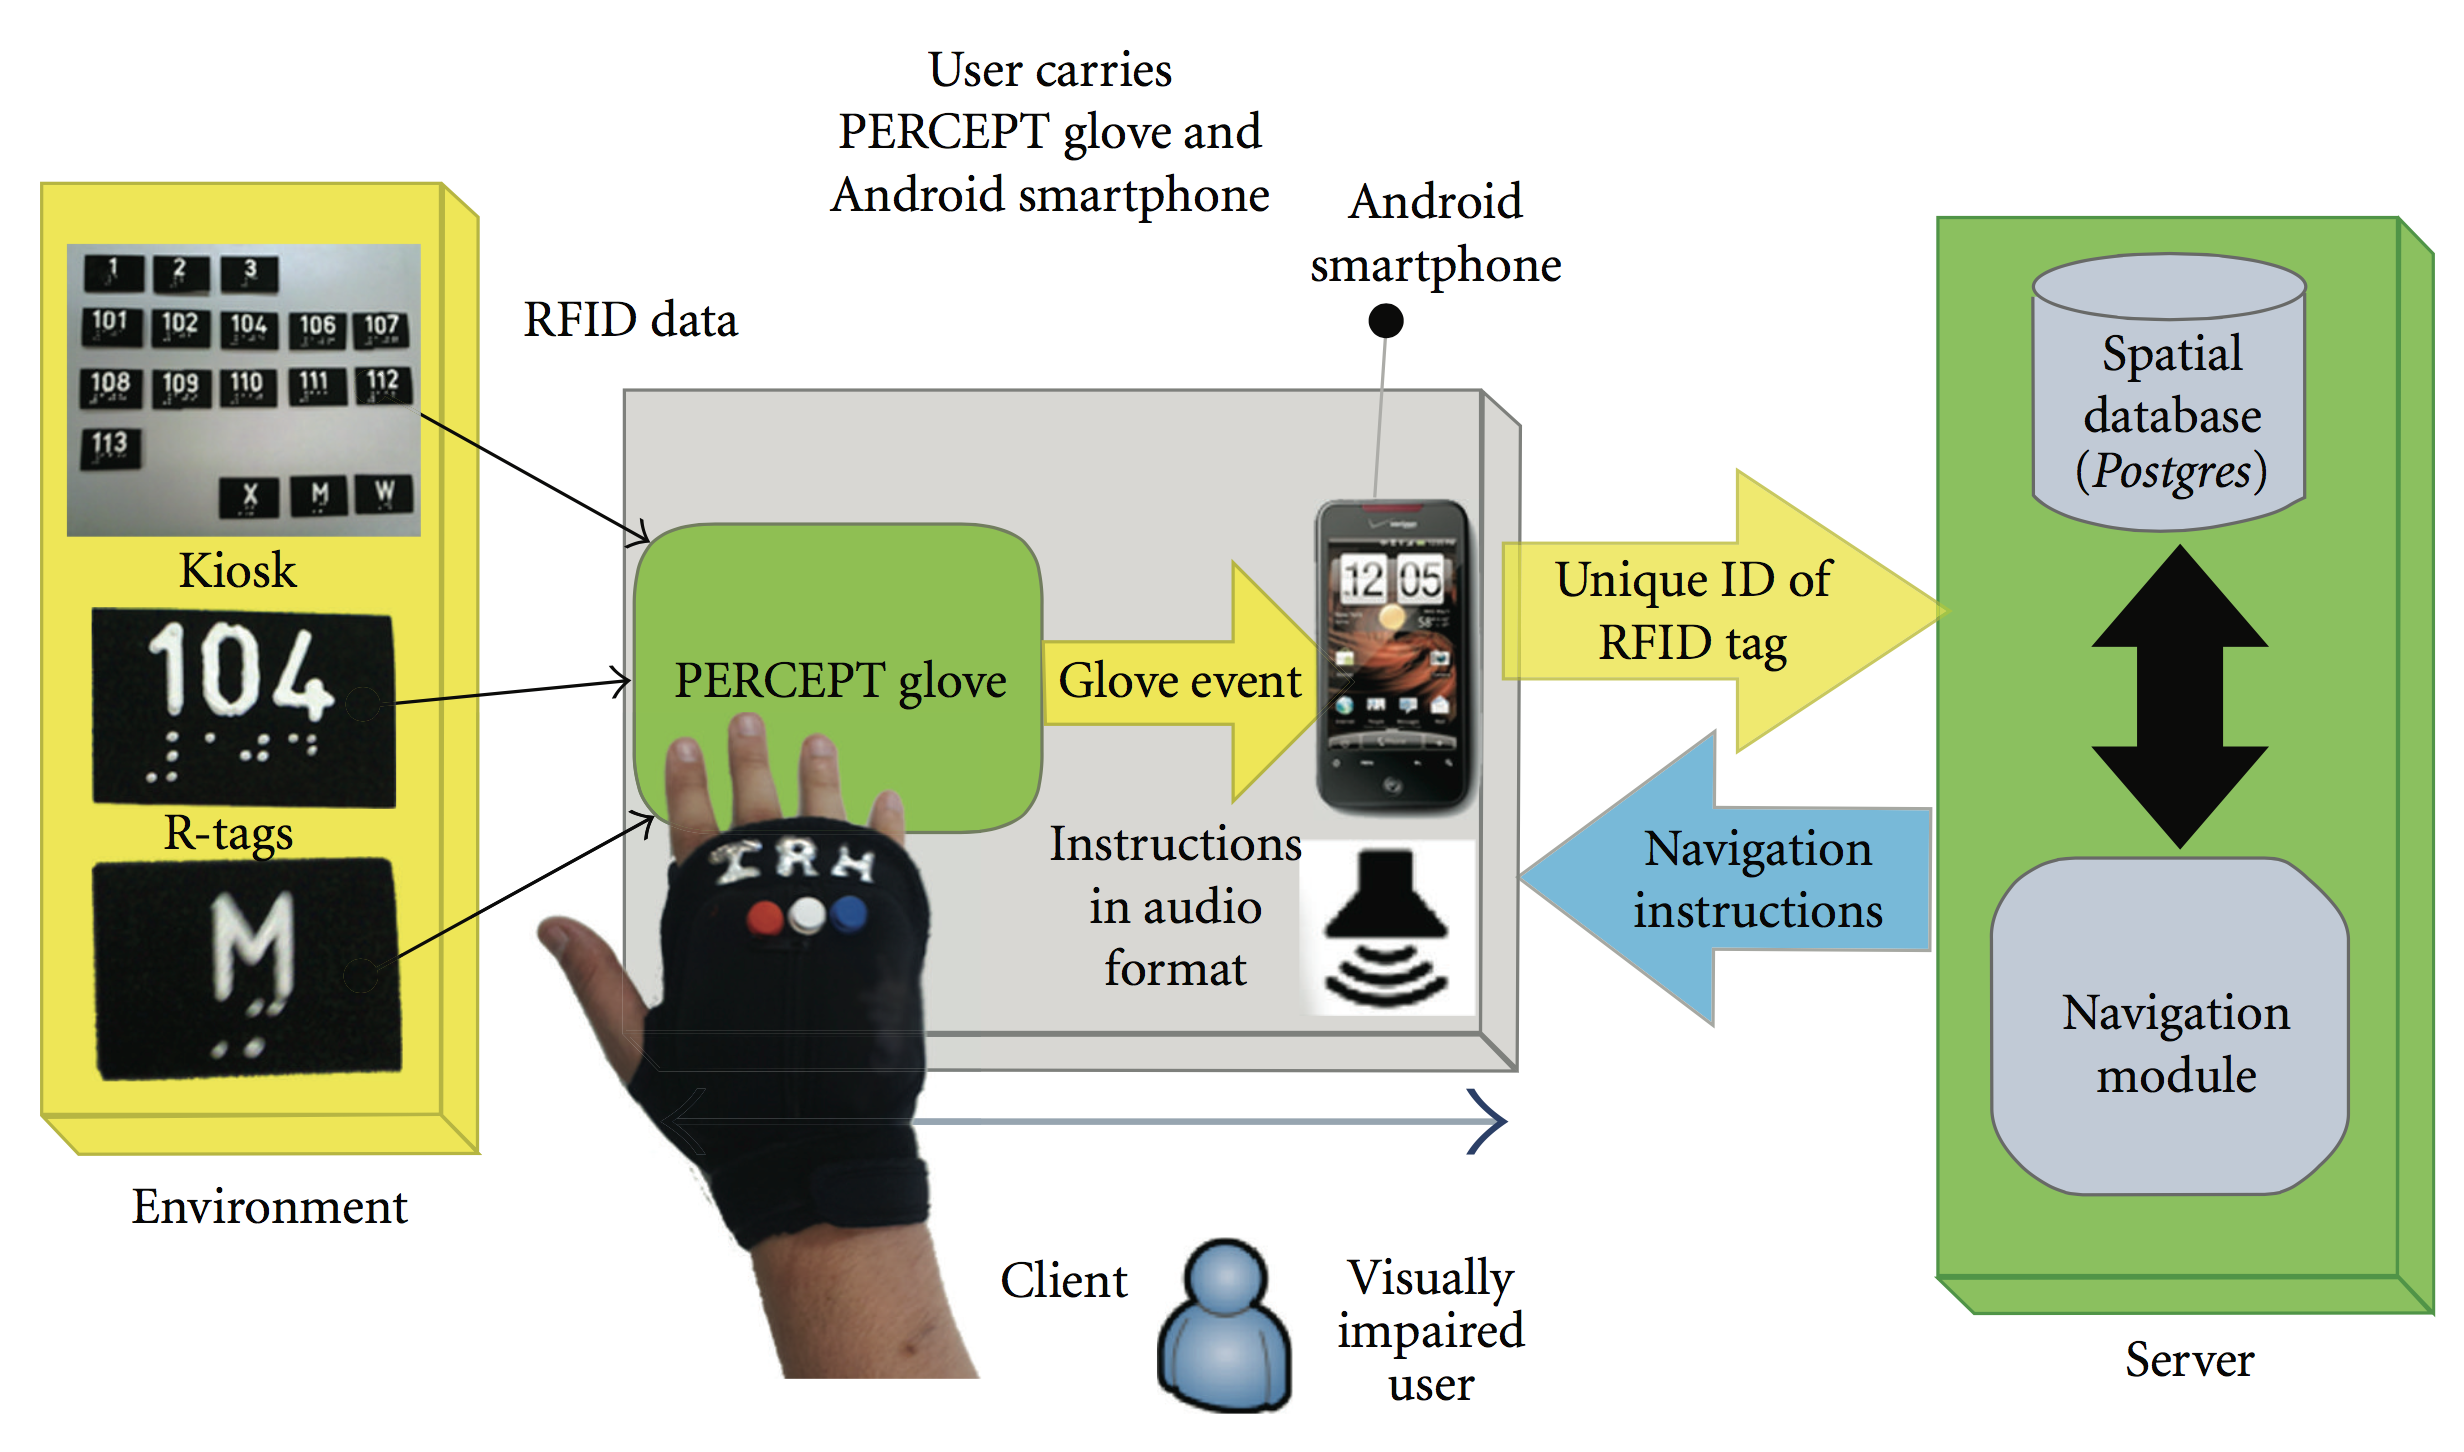
\includegraphics[width=\textwidth]{imgs/perceptArquitetura}
			\fonte{\citetexto{Ganz2011}}
		\end{minipage}
	\end{figure}
\FloatBarrier

Em uma breve avaliação do modelo, podemos ressaltar que, devido ao baixo custo das tags RFID, é fácil implantar o sistema em um grande ambiente. Porém, a necessidade de conexão constante com a internet pode ser um problema. O fato de o usuário necessitar procurar os quiosques, bem como encontrar a tag correspondente ao destino desejado, é um grande complicador.

%=======================================================================
% TIRÉSIAS
%=======================================================================
	\section{Tirésias}
Em \citetexto{Falk2013} é proposto um modelo para acessibilidade chamado Tirésias. De acordo com o artigo, o Tirésias é baseado no Hefestos. Este, por sua vez, é um modelo genérico que visa procurar estabelecer alguns padrões de acessibilidade que possam ser aplicados em diversos tipos de deficiência. Segundo os autores, o Tirésias pode ser compreendido como uma especialização construída em cima do modelo Hefestos para atender as necessidades das pessoas com deficiência visual. 

De acordo com \citetexto{Falk2013}, o Tirésias emprega conceitos de sensibilidade ao contexto e acessibilidade ubíqua, utilizando maneiras especializadas de interação com o sistema, para promover acessibilidade a PDV. Dessa forma, o modelo é capaz de oferecer informações relevantes ao contexto onde o usuário está e o que existe a sua volta.

O Tirésias funciona obtendo informações de localização do usuário através do GPS contido no smartphone e, baseado nisso, o sistema exibe recursos de acessibilidade disponíveis nas proximidades do usuário. Algumas das funcionalidades oferecidas são a listagem de recursos disponíveis, a indicação de caminho até recurso selecionado e a solicitação de ajuda.

O modelo Tirésias é composto pelos módulos de saída, entrada, configurações e pelo assistente pessoal, somados ao modelo Hefestos. A figura \ref{fig:visaoGeralTiresias} exibe uma visão geral da arquitetura do Tirésias, mostrando em cima os componentes do próprio modelo, e embaixo os componentes do modelo em que ele é baseado. Os componentes são descritos abaixo.

\begin{figure}
	\caption{Visão geral da arquitetura do Tirésias}
	\label{fig:visaoGeralTiresias}
	\centering%
	\begin{minipage}{.6\textwidth}
		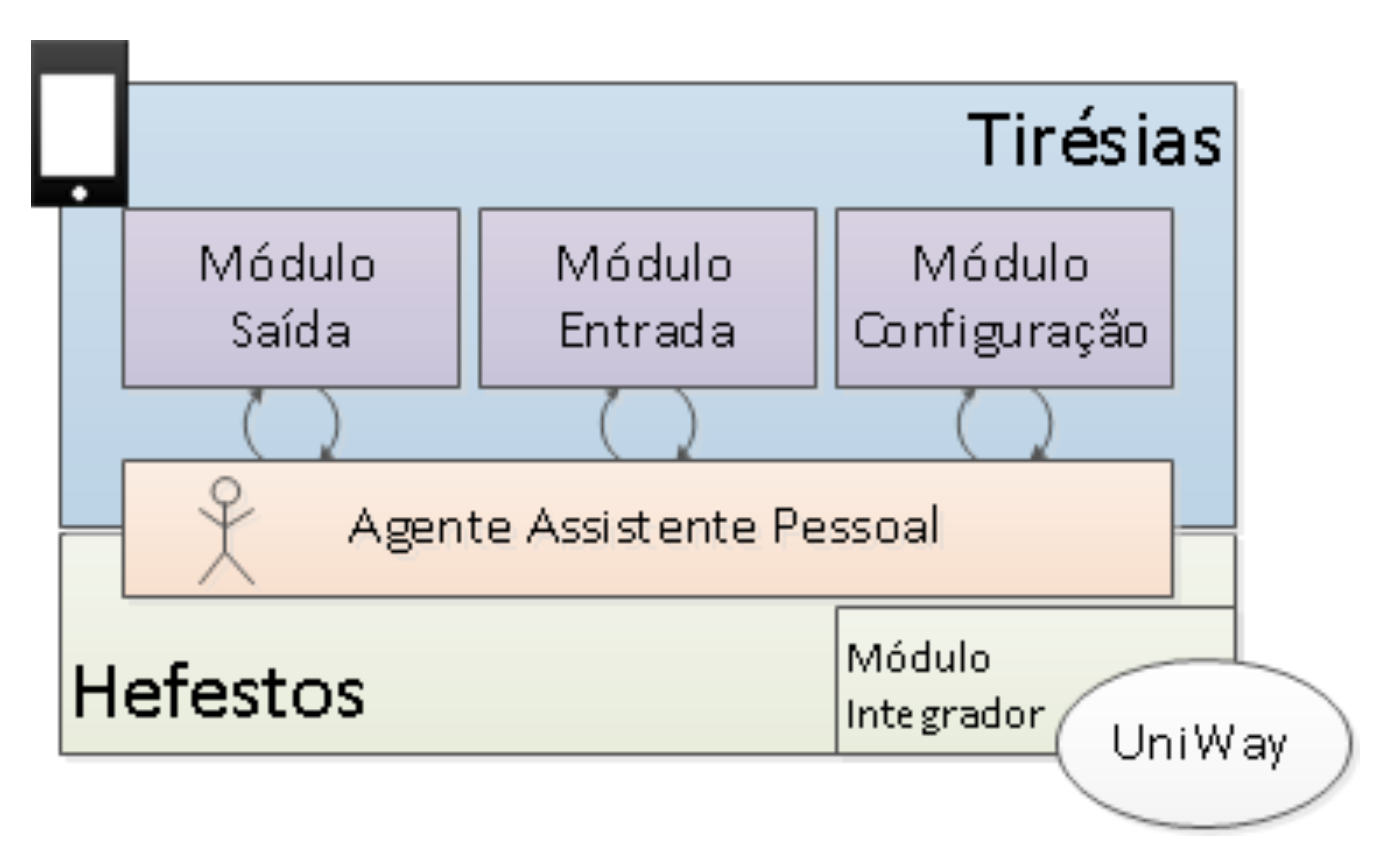
\includegraphics[width=\textwidth]{imgs/tiresiasArquitetura}
		\fonte{\citetexto{Falk2013}}
		\end{minipage}
\end{figure}

\begin{itemize}
	\item O módulo de saída é o responsável por gerenciar as informações passadas aos usuários. Informações são divididas em dois grupos: o primeiro são indicações de recursos disponíveis próximos ao usuário; o segundo tipo são os trechos do caminho até um determinado destino escolhido pelo usuário. Para comunicar as informações ao usuário, são utilizados a leitura da tela em conjunto com alertas vibratórios. A disponibilização das informações do primeiro tipo envolve a leitura do nome, da descrição e da distância até cada recurso um dos recursos disponíveis, baseado na posição atual do usuário. Conforme o usuário de movimenta, a informação de distância dos recursos é atualizada. A diferença do segundo tipo é que apenas o destino parcial mais próximo é disponibilizado e, quando o usuário conclui o trecho atual, o próximo é lido. Além da leitura de tela, o Tirésias combina a utilização de alertas vibratórios com a bússola eletrônica que equipa os smartphone para indicar a direção correta aos usuários. Quando o smartphone está voltado em direção do próximo destino, o fato é informado ao usuário através de vibrações, interrompidas quando o smartphone é virado para outras direções.

	\item O módulo de entrada gerencia a interface do usuário com o sistema. Capaz de suportar dispostivos com teclado dedicado ou somente a tela sensível ao toque, o Tirésias se adapta aos recursos disponíveis no smartphone para oferecer a maneira mais conveniente de interação ao usuário. É através deste módulo que o usuário informa ao modelo onde deseja ir, por exemplo.

	\item O módulo de configuração disponibiliza o controle de ajustes de todas as funcionalidades disponíveis no sistema, de forma a customizar o sistema às necessidades de diferentes usuários. Alguns dos ajustes disponíveis são o controle de frequência e volume da leitura de tela, a quantidade de recursos lida e se o usuário deseja ser notificado quando há alguma mudança nos recursos.

	\item O agente é responsável pela comunicação com o Hefestos, através da qual são obtidos perfis de usuários e recursos disponíveis para o suporte à acessibilidade.
\end{itemize} 

Avaliando o modelo, é notável a acessibilidade no que tange a entrada e saída dos dados no aplicativo. Entretanto, um ponto fraco é a utilização do GPS como modo de localização, visto que o sistema é incapaz de identificar um andar específico em um prédio com muitos pisos, por exemplo, bem como o sinal pode ser fraco ou estar indisponível em algumas regiões devido à natureza da tecnologia. 

%=======================================================================
% UCAT
%=======================================================================
	\section{UCAT - Ubiquitous Context Awareness Tools for the Blind}
\citetexto{ucat2014} apresenta uma pesquisa cujo objetivo é identificar as necessidades de informação de um deficiente visual, focando principalmente em questões relacionadas a percepção, orientação em ambientes conhecidos e desconhecidos e também em dificuldades comumente enfrentadas no dia-a-dia, após algumas entrevistas com PDV o trabalho descobriu que a falta de conhecimento a respeito das pessoas ao redor foi apontada como a principal causa de desconforto. Além disso, todos os entrevistados afirmaram que seria muito bom possuir uma ferramenta sutil e discreta que os ajudasse a obter mais informações sobre seus arredores.

O autor afirma que não existe nenhum sistema que forneça a usuários cegos informações sobre o contexto ao seu redor e propõe um modelo com essa finalidade. Desenvolvido para dispositivos móveis que suportam a tecnologia Bluetooth, objetiva ser uma ferramenta através da qual os PDV podem criar, compartilhar e receber informações a respeito de pessoas, locais ou objetos através de notas. 

Usando Bluetooth como ferramenta de detecção e o endereço MAC do dispositivo para identificar unicamente cada telefone, a aplicação mostra todos os dispositivos ao redor do usuário, sendo capaz de detectar quando alguém se aproxima ou se afasta. O sistema permite criar contatos, associando aparelhos de telefone a pessoas específicas, permitindo também que o usuário crie notas de texto ou voz relacionadas a alguém ou algum lugar. O modelo periodicamente busca por dispositivos próximos e, quando encontra algum, procura se alguma nota foi criada e associada a ele. Se uma associação é encontrada, o aplicativo notifica o usuário através de alertas vibratórios que podem ser personalizados.

Aqui existe um grande ponto fraco da tecnologia utilizada. Para funcionar corretamente, é necessário que todos os dispositivos estejam com o Bluetooth conectado e em modo visível aos demais; caso contrário, o aplicativo é incapaz de detectá-los.

A arquitetura do sistema possui estrutura cliente-servidor, onde o servidor é responsável apenas por hospedar a base de dados e trocar informações entre usuários através da ferramenta Google Cloud Messaging (GCM) \footnote{Ferramenta de mensageria do Google, para mais informações consultar a documentação da ferramenta em https://developer.android.com/google/gcm/index.html} que é usada quando um usuário decide compartilhar alguma informação com outros. O smartphone é o responsável pela execução da maior parte das funcionalidades do modelo. Nele, ficam armazenadas as informações pessoas de cada usuário, seus contatos, associações e notas criadas.

A figura \ref{fig:visaoGeralUCAT} exibe uma visão geral da arquitetura do modelo UCAT. Nela podemos ver que os clientes conectados ao servidor e ao GCM, enquanto a base de dados se conecta ao servidor e ao GCM. 

\begin{figure}
	\caption{Visão geral da arquitetura do UCAT}
	\label{fig:visaoGeralUCAT}
	\centering%
	\begin{minipage}{.6\textwidth}
		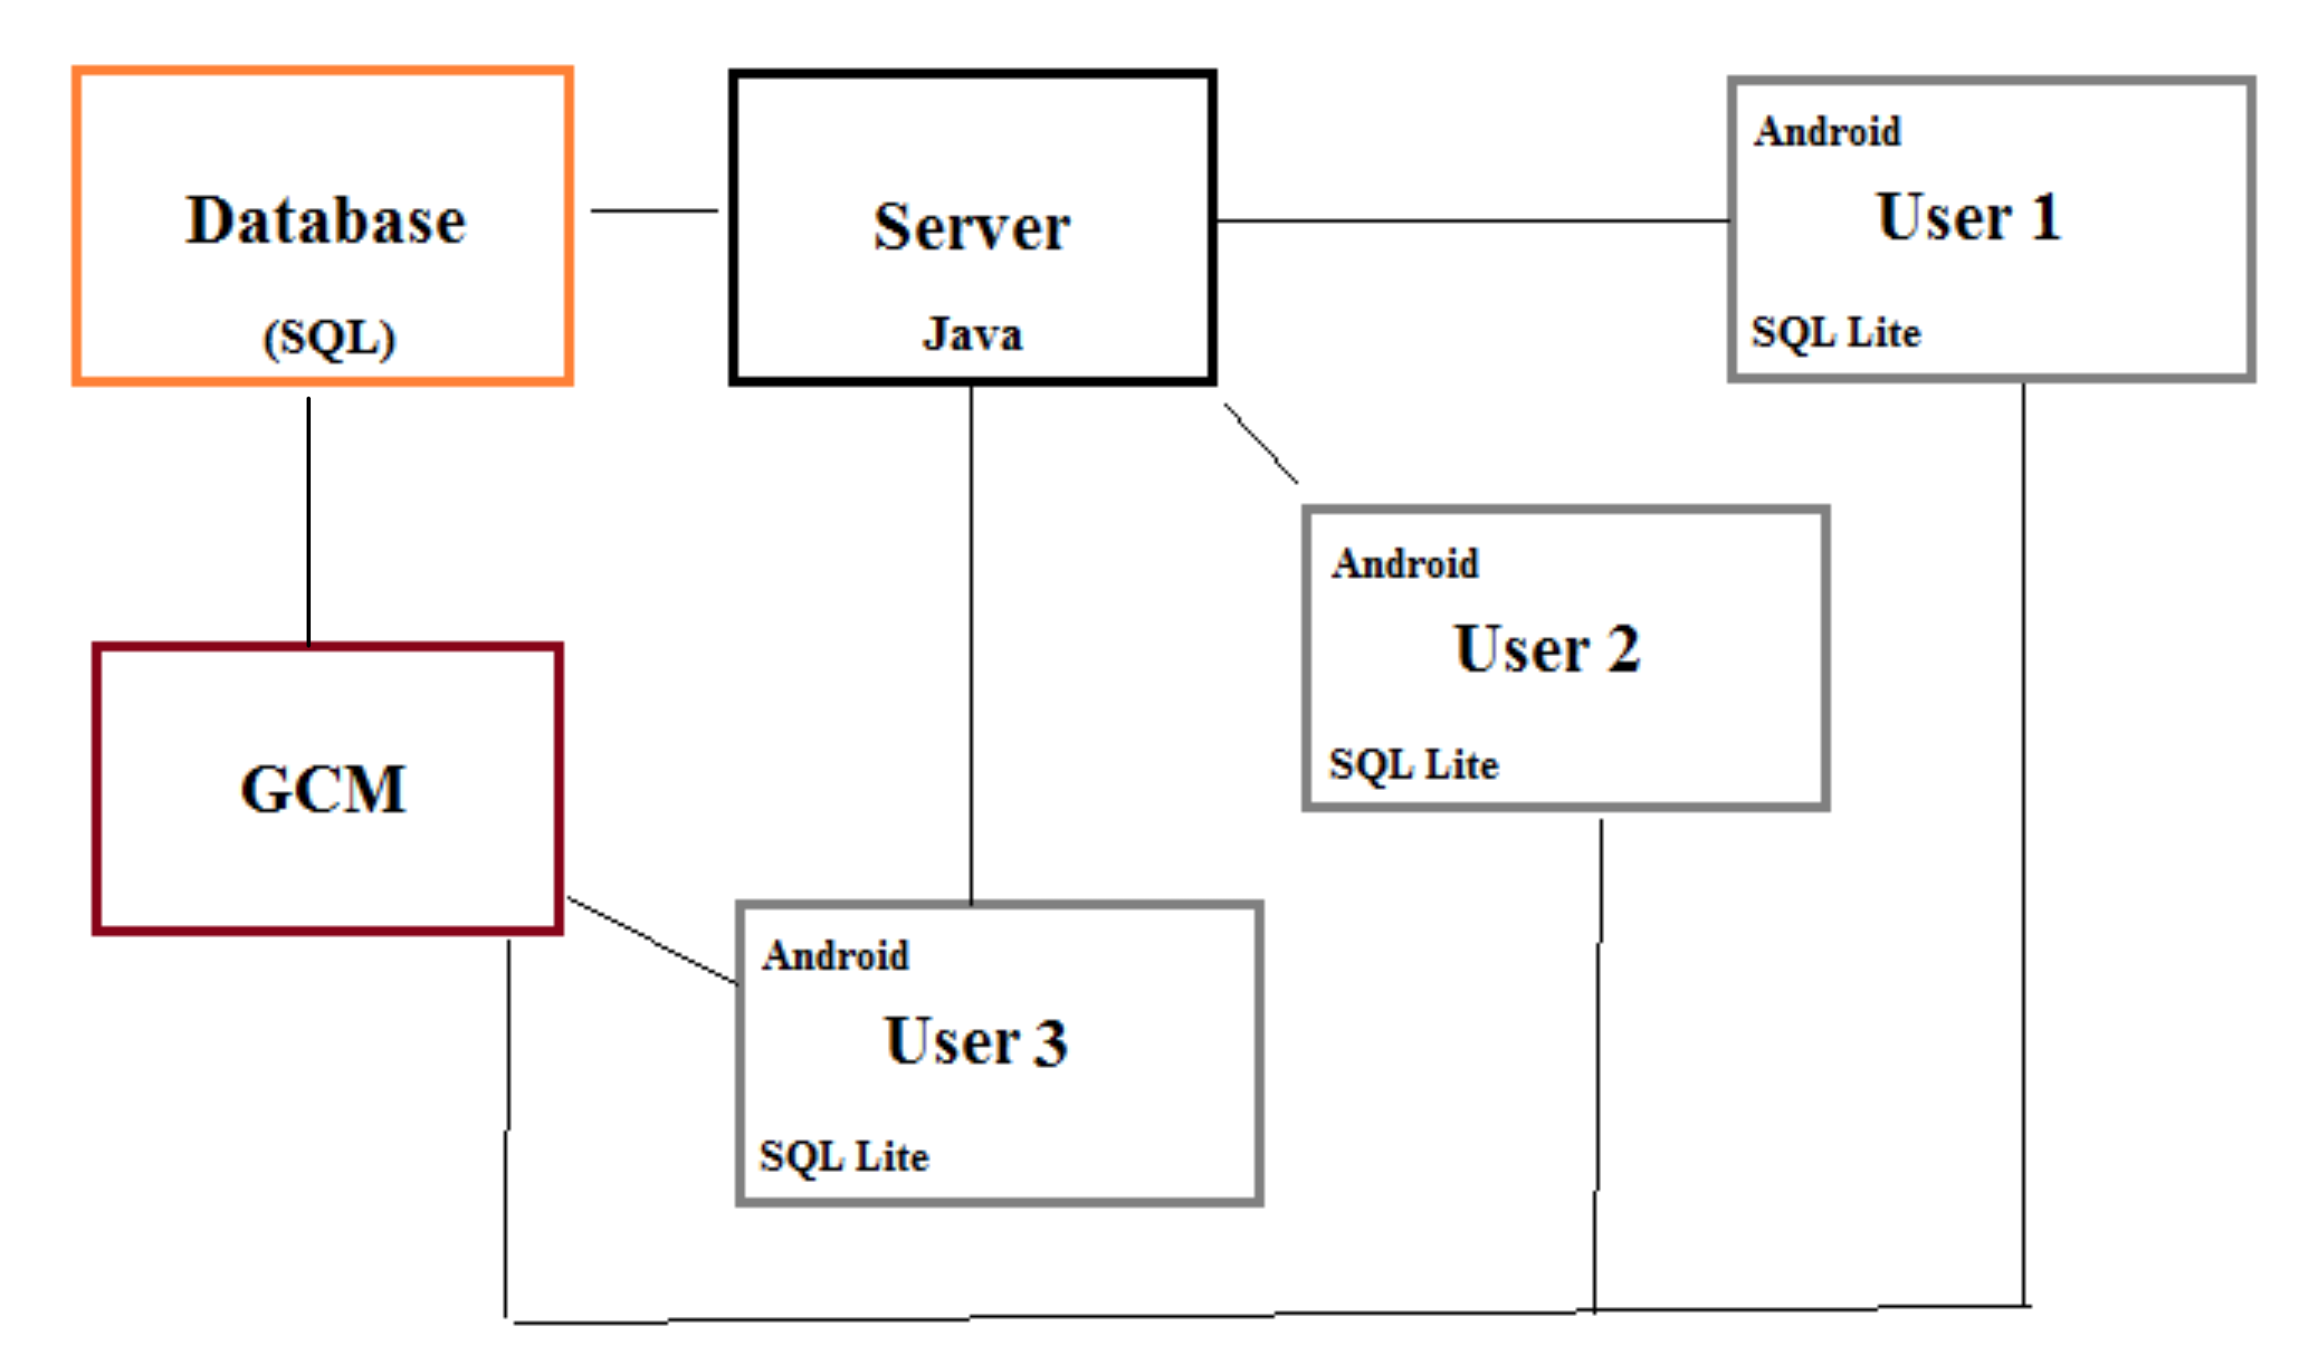
\includegraphics[width=\textwidth]{imgs/ucatArquitetura}
		\fonte{\citetexto{ucat2014}}
		\end{minipage}
\end{figure}

Para facilitar a interação dos usuários com o telefone, o sistema lança mão de alguns recursos de acessibilidade:
\begin{itemize}
	\item O sistema oferece diferentes formas de navegação baseada em gestos realizados na tela, afim de simplificar a navegação do usuário pelas telas e menus. Alguns gestos disponíveis são o deslizar, o clique duplo e o clique longo. O primeiro tem a função de percorrer as listagens de recursos e menus do aplicativo baseado na direção deslizada na tela. Já os outros servem para confirmar ações ou obter mais informações, respectivamente.
	
	\item Feedback por áudio, ou retorno do sistema através de voz, acontece através da função de conversão de texto para voz nativa do Android\footnote{Mais informações no Centro de Ajuda sobre acessibilidade do Android, em https://support.google.com/accessibility/android/}, sendo empregado para avisar ao usuário em que parte da aplicação ele se encontra, bem como listar funcionalidades de cada tela.

	\item Feedback tátil, ou alertas vibratórios, faz com que cada tipo de notificação emitida pelo sistema seja acompanhada por um padrão diferente de vibração, de modo a permitir que o usuário entenda o motivo do alerta sem obrigá-lo a retirar o telefone do bolso.
\end{itemize}

%=======================================================================
% BLUETOOTH WORKZONES
%=======================================================================
	\section{Development of a Navigation System Using Smartphone and Bluetooth Technologies to Help the Visually Impareid Navigate Work Zones Safely} 

O estudo realizado por \citetexto{chen2014} revela que pedestres correspondem a 17\% das mortes em canteiros de obras nos Estados Unidos. Segundo o autor, um grande planejamento é feito para acomodar o trafego de pedestres ao redor de zonas em obras, especialmente para os deficientes visuais, e garantir segurança no trajeto. O trabalho descreve seus objetivos da seguinte forma: compreender quais as informações relevantes para redirecionar PDV ao redor de obras, afim de prover mensagens relevantes e criar um sistema para dispositivos móveis afim de antecipadamente alertar seus usuários sobre a aproximação dos canteiros de obra. Ainda é citada a intenção de padronizar o formato de mensagens emitido em zonas em construção no redirecionamento dos transeuntes, afim de garantir aos PDV a possibilidade de caminhar independentemente e com segurança.

Para atingir o primeiro objetivo, foram conduzidas entrevistas com PDV afim de compreender os desafios que eles enfrentam e quais são consideradas informações relevantes durante seu deslocamento. Para o segundo objetivo, o trabalho propõe um aplicativo para smartphones Android que verbalmente emite mensagens enquanto seu usuário se aproxima das áreas delimitadas, fazendo uso de GPS, Bluetooth, função de conversão texto para voz e sensores presentes no telefone. 

\FloatBarrier
\begin{figure}
	\caption{Visão geral da arquitetura do modelo}
	\label{fig:visaoGeralWorkzones}
	\centering%
	\begin{minipage}{.6\textwidth}
		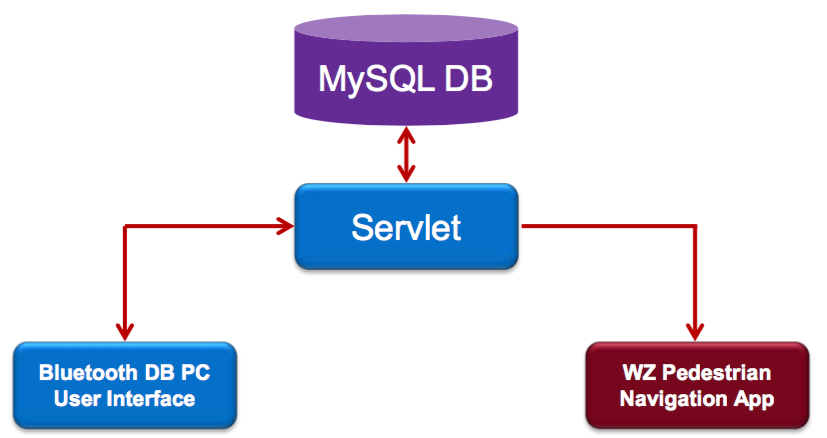
\includegraphics[width=\textwidth]{imgs/workzoneArquitetura}
		\fonte{\citetexto{chen2014}}
		\end{minipage}
\end{figure}
\FloatBarrier

O modelo consiste em três componentes: servidor com banco de dados com mapas, aplicativo para Android e beacons Bluetooth, 
\begin{itemize}
	\item O servidor contém o banco de dados onde ficam armazenados os mapas para referência espacial, informações sobre o posicionamento dos beacons e mensagens correspondentes a cada um deles. Essas informações são inseridas no banco de dados através de uma interface web acessada de um computador comum. O modelo de dados de cada beacon compreende um identificador único, latitude, longitude e nome do ponto onde ele foi posicionado e também quatro possíveis textos livres, de acordo com a estrutura das mensagens.

	\item O aplicativo constantemente busca por sinais Bluetooth nas proximidades do usuário. Quando algum é encontrado, seu identificador é comparado com aqueles cadastrados na base de dados espacial. Caso o aplicativo detecte que o usuário se encontra próximo a uma zona em obras, o telefone vibra e o alerta correspondente é emitido verbalmente através da função Text to Speech (TTS) do Android. É também função do aplicativo conectar-se periodicamente ao banco de dados afim de sincronizar sua base de dados local, mantendo as informações atualizadas. Apenas zonas num raio de até oito quilômetros do usuário são possíveis para garantir o funcionamento mesmo durante um breve período sem conexão com a base.
	
	\item Utilizados devido a possíveis problemas com o sinal GPS fraco ou inexistente, os beacons Bluetooth Smart podem ser posicionados nos limites das zonas em obras, em cavaletes ou cones, conforme mostrado na figura \ref{fig:workzoneScheme}. São dispositivos de baixo consumo que constantemente emitem seu identificador em um raio de dez metros, podendo ainda ser aumentado ou diminuindo conforme a necessidade.
\end{itemize}

A figura \ref{fig:visaoGeralWorkzones} mostra a arquitetura do modelo. Nela é possível ver que a base de dados é exposta através de um servidor, sendo acessada pelo aplicativo para obter as informações e por uma outra interface através de uma pagina web usada para manter as informações.

\FloatBarrier
\begin{figure}
	\caption{Demonstração da disposição dos beacons ao redor de uma zona em obras}
	\label{fig:workZoneScheme}
	\centering%
	\begin{minipage}{.4\textwidth}
		\includegraphics[width=\textwidth]{imgs/workzoneSchema}
		\fonte{\citetexto{chen2014}}
		\end{minipage}
\end{figure}
\FloatBarrier

As mensagens emitidas pelo aplicativo seguem o padrão estabelecido durante as entrevistas, sendo formadas por quatro partes distintas \cite{chen2014}:
\begin{itemize}
	\item Breve anúncio para chamar atenção do usuário
	\item Localização atual
	\item O que e onde
	\item Ação recomendada
\end{itemize}

Uma mensagem de exemplo, seguindo esse padrão, poderia ser: Atenção, você está na esquina da Rua X com a Rua Y, a calçada encontra-se fechada por Z metros. Atravesse a rua X para receber mais informações.

O pronto fraco desse trabalho é a baixa área de abrangência da solução, funcionando apenas no entorno de zonas em obras.
A pesquisa e a tecnologia seriam melhores aproveitadas em situações mais corriqueiras, como em um ambiente de uma universidade ou um estádio. Vale citar como ponto forte o uso da ultima versão da tecnologia Bluetooth, ao contrário dos outros trabalhos citados, onde não é necessário parear os dispositivos para que eles se comuniquem.

	\section{Comparação entre os trabalhos estudados}\label{comparacaoTrabs}

Com o intuito de facilitar a compreensão e a comparação dos trabalhos relacionados, um comparativo entre os trabalhos foi traçado. A partir do comparativo, a tabela \ref{tab:trabalalhosRelacionados} foi desenvolvida, contendo os principais dados sobre os modelos estudados. Nela são apresentadas as abordagens usadas em cada um dos modelos, sendo possível identificar de forma ágil as características e tecnologias aplicadas em cada um, permitindo a identificação de pontos fortes e lacunas relevantes para o presente trabalho. 

Alguns critérios foram selecionados para uma comparação mais clara entre os trabalhos, cada item da tabela se relaciona com um critério considerado nos modelos selecionados: o método de localização diz respeito a tecnologia utilizada pelo modelo para obter a localização do usuário; a abrangência se refere ao tipo de ambiente em que o modelo se propõe a funcionar; ambientes dinâmicos indica a capacidade do modelo de lidar com mudanças no ambiente; hardware específico demonstra se o modelo exige que o usuário carregue consigo mais um equipamento ou se o modelo se encaixa em um equipamento já existente; comunicação descreve a maneira utilizada pelo modelo para se comunicar com servidores ou atores externos; interoperabilidade mostra se o modelo prevê que seus dados possam ser utilizados por outras aplicações; banco de dados, linguagem e sistema operacional descrevem quais tecnologias são usadas pelo modelo durante seu desenvolvimento e uso; hardware diz especificamente qual o aparato que o usuário deverá possuir para utilizar o modelo; por fim, arquitetura descreve os componentes de software do modelo e a forma com que eles se comunicam.

Os aspectos mais relevantes na comparação são o hardware que é utilizado no modelo, a tecnologia aplicada na determinação da localização do usuário e a área de abrangência do sistema. Todos os modelos estudados são focados no uso de dispositivos móveis, no entanto, um deles exige o uso combinado de outro dispositivo de hardware dedicado. Dois dos trabalhos utilizam Bluetooth para obter a localização, enquanto os outros usam RFID ou GPS. Em relação ao último aspecto, três dos sistemas possuem foco em ambientes internos, enquanto um é mais específico e voltado a zonas em construção.

\FloatBarrier
\begin{table}
	\caption{Tabela comparativa entre os trabalhos relacionados}
	\label{tab:trabalalhosRelacionados}
	\centering%
	\begin{minipage}{1\textwidth}
		\begin{tabular}{ p{3cm} | p{3cm} | p{3cm} | p{3cm} | p{3cm} }
			\hline
										& Percept 									& UCAT 								& Navigation System for Work Zones		& Tirésias   \\ \hline
				Método de localização 	& RFID 										& Bluetooth 2.1 					& Bluetooth 4.0 						& GPS 						 \\ \hline
				Abrangência 			& Indoor 									& Indoor e outdoor 					& Zonas em obras 						& Indoor 					 \\ \hline
				Ambientes dinâmicos		& Não especificado							& Não especificado					& Não especificado						& Não especificado			 \\ \hline
				Hardware específico 	& Sim 										& Não 								& Não 									& Não 						 \\ \hline
				Comunicação 			& Internet ou intranet 						& Internet 							& Internet 								& Internet ou intranet 		 \\ \hline
				Interoperabilidade 		& Não 										& Não 								& Não 									& Sim 						 \\ \hline
				Banco de dados 			& Postgres 									& SQLite 							& MySQL 								& Não especificado 			 \\ \hline
				Linguagem 				& Java 										& Java 								& Java 									& Objective-C 				 \\ \hline
				Sistema operacional 	& Android 									& Android 							& Android 								& iOS 						 \\ \hline
				Hardware 				& Luva equipada c/ leitor RFID e smartphone & Dispositivos móveis c/ Bluetooth 	& Dispositivos móveis c/ Bluetooth 		& Dispositivos Móveis c/ GPS \\ \hline
				Arquitetura 			& Cliente-servidor 							& Cliente-servidor 					& Cliente-servidor 						& Cliente-servidor 			 \\ \hline
		\end{tabular}
		\fonte{Elaborado pelo autor.}
	\end{minipage}
\end{table}
\FloatBarrier

No que tange a outros aspectos avaliados, a arquitetura de todos os modelos se assemelha no uso da estrutura cliente-servidor com comunicação via internet. Apenas o Tirésias foi desenvolvido em Objetive-C para a plataforma iOS, enquanto todos os outros foram desenvolvidos em Java para a plataforma Android. Ainda é possível ressaltar que apenas o Tirésias concebe interoperabilidade para outras aplicações que podem vir a ser desenvolvidas.

Foi identificado que nenhum dos modelos selecionados faz uso de bibliotecas ou frameworks que visem promover acessibilidade. Além disso, as tecnologias de localização usadas em três dos modelos não se adequam perfeitamente a ambientes internos, pois exigem proximidade muito grande do usuário para obter as informações ou então não são capazes de identificar múltiplos andares em um ambiente. O modelo destinado a áreas em construção é o único que faz uso da tecnologia mais adequada, o Bluetooth Low Energy. Porém, a emprega em uma área de abrangência muito pequena.
Outra lacuna identificada foi a falta de informações a respeito do gerenciamento, por parte dos modelos, de mudanças que possam acontecer eventualmente nos ambientes, ou ambientes dinâmicos. Por fim, foi identificado que o único modelo que considera a possibilidade integração com outras soluções é o Tirésias.























%=======================================================================
% Modelo proposto
%=======================================================================
\chapter{Modelo Proposto}
% Essa etapa consiste em detalhar o modelo. O capítulo do modelo deve começar a partir da delimitação da pesquisa, dizendo quais lacunas serão atacadas e como. Geralmente há uma visão geral do modelo aqui, já desenvolvido na atividade 4. Esse capítulo detalha como a questão de pesquisa será respondida? Que modelo computacional é necessário para isso. Se é proposta uma ontologia, ela é detalhada aqui; Se há um modelo de contexto, ele é detalhado aqui. Pode-se usar alguns diagramas para representar a arquitetura, interações, fluxos e componentes. Lembre-se que o modelo pode ter diferentes implementações e não precisa ser limitado por uma tecnologia específica. Por exemplo, não faz sentido dizer que o modelo é para Android ou feito em Java. Por que não poderia ser para iOS e feito em Objective C? Que característica de um modelo limitaria isso?

% Lacunas
% Visão geral
% Como a questão de pesquisa será respondida
% Diagramas (arquitetura, interações, fluxos e componentes)

Este capítulo apresenta um modelo de sistema que visa promover acessibilidade de pessoas com deficiência visual. O modelo atua auxiliando na localização e no deslocamento de seus usuários, contando com recursos que facilitam sua interação, visto que PDV necessitam de formas especializadas de contato com dispositivos. \citetexto{Falk2013}.

O principal recurso agregado ao modelo é a utilização do kit de desenvolvimento de software indoo.rs, fornecido pela empresa Indoors. O indoo.rs promove acessibilidade buscando ser a base na qual são montadas aplicações que necessitam de informações precisas e em tempo real. A decisão de usar essa biblioteca se deve ao fato de o kit facilitar o desenvolvimento de soluções de localização, tanto para aparelhos Android quanto para aparelhos iOS, através de beacons Bluetooth. Outras características da plataforma indoo.rs são a dispensa da necessidade de conexão com a internet, o baixo consumo de energia e a inclusão de ferramentas analíticas e gerenciais, através das quais é possível extrair inúmeras informações a respeito do movimento dos usuários nas premissas do ambiente. Outros diferenciais do modelo são a utilização de sensibilidade ao contexto e o suporte às funcionalidades de acessibilidade, oferecidas nativamente pelos sistemas operacionais.
São previstos também o suporte a ambientes dinâmicos e a possibilidade de integração com outras soluções, ambos através de um serviço web.

\section{Visão geral do modelo} 
O modelo, batizado de Insight, foi concebido tendo em mente tecnologias existentes e já disponíveis ao alcance da maioria das pessoas. Todos os equipamentos necessários já existem no mercado, de forma que não é preciso fazer modificações em produtos, ou usar hardware dedicado para aproveitar as funcionalidades aqui descritas.

O objetivo do modelo é promover acessibilidade aos seus usuários, possibilitando que eles estejam sempre cientes dos recursos ao seu redor e do caminho até eles. Para isso, o aplicativo auxília o usuário em seu deslocamento curva-a-curva através de instruções verbais. No entanto, visto que o objetivo do modelo não é alertar sobre obstáculos no caminho do usuário, ele não deve ser visto como um substituto para ferramentas que possuam esse fim. O Insight deve ser sempre usado em conjunto com outras ferramentas assistivas, tais como bengalas e cães guia, esses sim possibilitam o desvio de quaisquer obstáculos que possam surgir. 

Empresas ou organizações que queiram melhorar a acessibilidade de suas dependências devem ter em mente que outras medidas podem ser tomadas em conjunto com a adoção do modelo, para aumentar a eficiência de seus esforços. Uma medida que possui sinergia total com o Insight é a colocação de piso tátil por todos os trajetos que serão percorridos pelos PDV. Piso tátil são faixas em auto-relevo no chão, fornecendo auxílio e indicações aos PDV durante seus deslocamentos.

A combinação Insight e piso tátil é bastante útil no empoderamento e independência dos usuários. Através do Insight é possivel descobrir locais e rotas, e através do piso tátil os usuários podem ter certeza de que o caminho sendo percorrido é seguro e não possui obstáculos que dificultem o trânsito.

O modelo é composto por um aplicativo para dispositivos móveis, um servidor e diversos beacons Bluetooth, conforme mostrado na figura \ref{fig:visaoGeral}. 

O aplicativo contempla os seguintes módulos: serviço Bluetooth, motor de localização, módulo de saída, módulo de sincronização e base secundária. No servidor ficam hospedados um serviço web REST, uma ferramenta de gerenciamento dos ambientes e uma base de dados primária. Os beacons serão previamente distribuídos em pontos-chave do local onde o modelo for aplicado, de forma a otimizar seu alcance e área de cobertura.

Através do modelo, o usuário poderá saber onde está, descobrir recursos que existem a sua volta e selecionar algum recurso específico para que seja traçada uma rota para chegar ao destino escolhido, entre outras funcionalidades. O aplicativo fornece instruções via áudio e alertas vibratórios, através dos recursos assistivos dos smartphones, para guiar o usuário conforme avança pelo caminho até o seu destino.

Cada um dos componentes, bem como a arquitetura do modelo, são explicados em maiores detalhes nas seções subsequentes.

\begin{figure}
	\caption{Visão geral do modelo}
	\label{fig:visaoGeral}
	\centering%
	\begin{minipage}{.8\textwidth}
		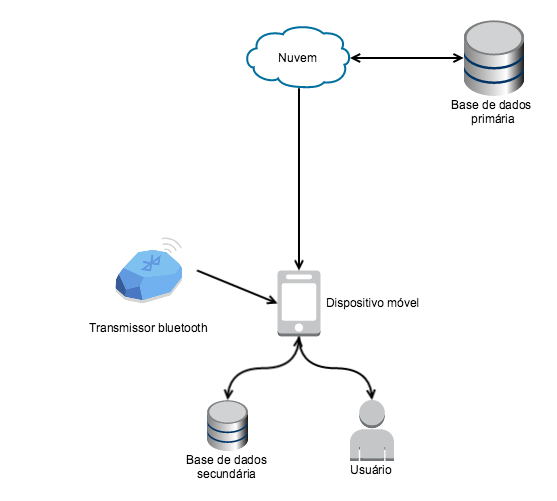
\includegraphics[width=\textwidth]{imgs/visaoGeral}
		\fonte{Elaborado pelo autor.}
	\end{minipage}
\end{figure}

	\section{Requisitos e casos de uso}
O diagrama de casos de uso apresentado na figura \ref{fig:diagramaCasosDeUso} foi desenvolvido para auxiliar na fase de elicitação de requisitos, fornecer uma melhor visualização das funcionalidades da solução, e também mostrar quais são os atores envolvidos com cada uma delas. O diagrama foi construído levando em consideração as características encontradas nos trabalhos relacionados, bem como as informações presentes no referêncial teórico deste trabalho.

	\begin{figure}
		\caption{Diagrama de casos de uso do Insight}
		\label{fig:diagramaCasosDeUso}
		\centering%
		\begin{minipage}{,9\textwidth}
			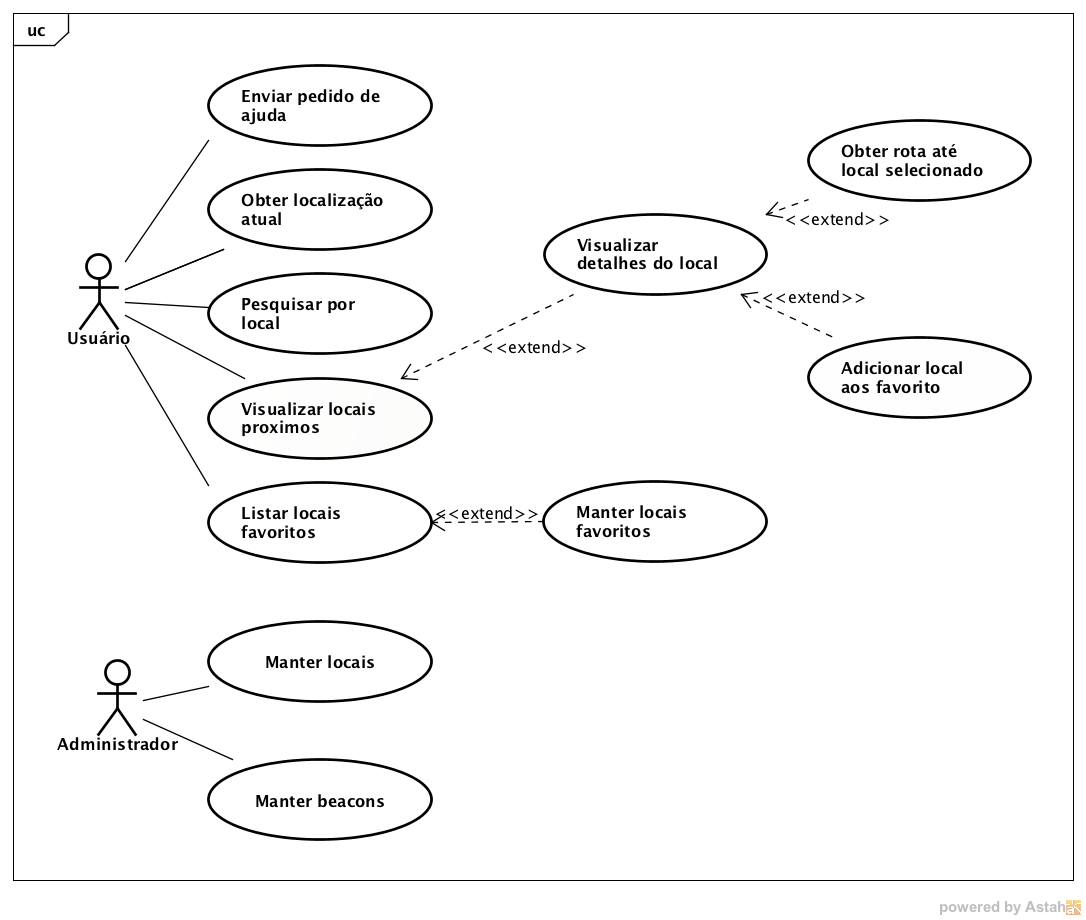
\includegraphics[width=\textwidth]{imgs/casosDeUso}
			\fonte{Elaborado pelo autor.}
		\end{minipage}
	\end{figure}

A listagem dos requisitos é apresentada nas seções subsequentes, sendo dividida entre requisitos funcionais e requisitos não funcionais.

\subsection{Requisitos funcionais} 
Nesta seção são apresentados os requisitos funcionais elicitados para o modelo Insight. Cada requisito funcional corresponde a uma funcionalidade presente na solução, afim de que usuários possam desempenhar suas ações. Para a definição dos requisitos foi levado em consideração que o sistema possui dois tipos de usuários: usuários comuns e administradores.

Os requisitos funcionais elicitados para o modelo são:

	\begin{itemize} % breve descrição, atores, condições previas, fluxo de eventos (basico e alternativo), pós condições 
		% USER
		\item \textbf{RF01 - Obter localização atual:} o usuário poderá obter sua localização atual a qualquer momento.
		
		\item \textbf{RF02 - Visualizar locais próximos:} o usuário poderá visualizar os locais próximos a si, ordenados pela distância até o local.
		
		\item \textbf{RF03 - Pesquisar por local:} o usuário poderá pesquisar entre os locais disponíveis usando critérios como nome ou categoria.
		
		\item \textbf{RF05 - Visualizar detalhes do local:} o usuário poderá visualizar informações específicas do local selecionado, tais como nome, descrição, categoria e distância até ele.

		\item \textbf{RF08 - Obter rota até local selecionado:} o usuário poderá obter uma rota até o local selecionado, partindo do seu local atual.

		\item \textbf{RF04 - Listar locais favoritos:} o usuário poderá visualizar uma lista com os locais marcados como seus favoritos.
		
		\item \textbf{RF06 - Manter locais favoritos:} o usuário poderá adicionar ou excluir locais da lista de locais favoritos.
		
		\item \textbf{RF09 - Enviar pedido de ajuda:} o usuário poderá enviar aos administradores um pedido de ajuda informando o seu local atual, para que alguém seja enviado para socorrer o usuário.
		
		% ADMIN
		\item \textbf{RF10 - Manter locais:} o administrador poderá adicionar, editar, ou excluir locais cadastrados no modelo.
		
		\item \textbf{RF11 - Manter beacons:} o administrador poderá adicionar, editar, ou excluir beacons cadastrados no modelo.

	\end{itemize}

\subsection{Requisitos não funcionais}
Nesta seção são apresentados os requisitos não funcionais elicitados para o modelo Insight. Os requisitos não funcionais descrevem aspectos internos da aplicação no que diz respeito ao desempenho, confiabilidade, interoperabilidade, mobilidade, disponibilidade, segurança e usabilidade.

Os requisitos não funcionais elicitados para o modelo Insight são:

\begin{itemize}
	\item \textbf{RNF01 - Interoperabilidade - Usar servidor web:} O servidor será uma aplicação web.

	\item \textbf{RNF02 - Interoperabilidade - Serviços web REST:} o servidor disponibilizará serviços web utilizando o padrão Representational State Transfer (REST) para realizar a integração com os clientes e outras aplicações.

	\item \textbf{RNF03 - Interoperabilidade - JSON:} o sistema usará o padrão Javascript Object Notation (JSON) para a transferência de informações a partir do servidor REST, afim de facilitar a comunicação com os clientes e outras aplicações.

	\item \textbf{RNF04 - Portabilidade - Clientes para dispositivos móveis:} o sistema será utilizado em smartphones ou tablets.

	\item \textbf{RNF05 - Usabilidade - Base de dados secundária:} O aplicativo deverá conter uma cópia local do banco de dados do servidor.

	\item \textbf{RNF06 - Confiabilidade - Sincronização:} O aplicativo deverá periodicamente sincronizar sua base de dados com a base de dados do servidor.

	\item \textbf{RNF07 - Usabilidade - Adaptação ao contexto:} o sistema deverá identificar o contexto do usuário através do uso da localização, afim de exibir os recursos mais relevantes e fornecer os próximos passos da navegação.

	\item \textbf{RNF08 - Usabilidade - Comandos por gestos:} a aplicação deverá permitir a interação do usuário através de gestos.

	\item \textbf{RNF09 - Usabilidade - Comandos por voz:} a aplicação deverá permitir a interação do usuário através de comandos de voz.

	\item \textbf{RNF10 - Acessibilidade - Feedback por voz:} a aplicação deverá fornecer informações ao usuário através do uso de voz.

	\item \textbf{RNF11 - Acessibilidade - Feedback tátil:} a aplicação deverá fornecer informações ao usuário através do uso de alertas vibratórios.

	\item \textbf{RNF12 - Acessibilidade - Discrição:} o modelo deve poder ser utilizado a partir de hardware leve e discreto.

	\item \textbf{RNF12 - Usabilidade - Interferência:} o modelo não deve interferir em outras ferramentas que o usuário possa estar usando para se deslocar.
\end{itemize}

A partir dos requisitos funcionais e não funcionais, é possivel perceber que os dispositivos móveis são a ferramenta ideal para uso do modelo.

	\section{Arquitetura}
O Insight é projetado utilizando o modelo de arquitetura cliente-servidor. Os aplicativos cliente são instalados em dispositivos móveis, como smartphones e tablets, que se comunicam com o servidor através de serviços web. Para garantir que diversos usuários possam acessar o sistema ao mesmo tempo sem que a performance seja prejudicada, o servidor é disposto conforme o conceito de computação na nuvem, compartilhando os recursos físicos do servidor onde a aplicação está instalada. A figura \ref{fig:arquitetura} mostra um diagrama de blocos onde os principais componentes são exibidos, mostrando também as camadas em que a arquitetura do sistema está divida e como ocorre a troca de informações entre os componentes envolvidos. 

\FloatBarrier 
\begin{figure}
	\caption{Diagrama de blocos da arquitetura}
	\label{fig:arquitetura}
	\centering%
	\begin{minipage}{.8\textwidth}
		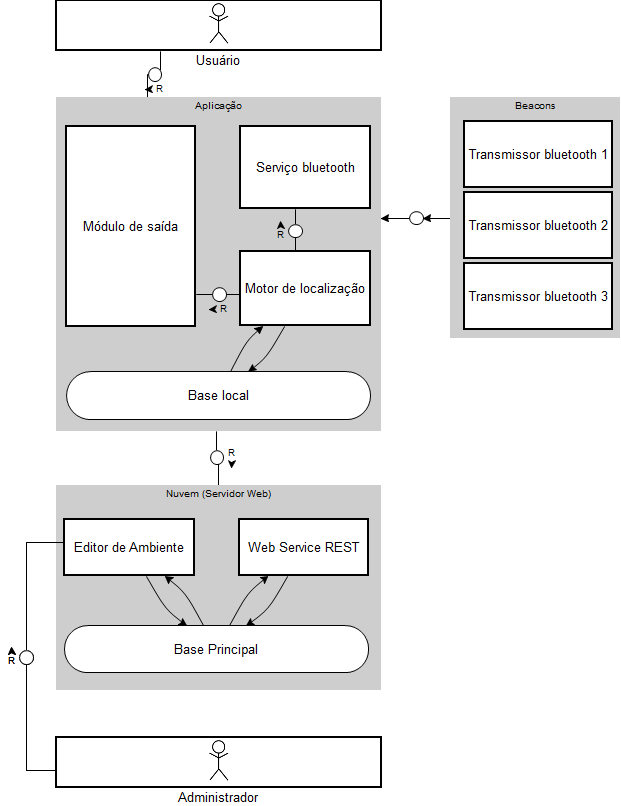
\includegraphics[width=\textwidth]{imgs/arquitetura.png}
		\fonte{Elaborado pelo autor.}
	\end{minipage}
\end{figure}
\FloatBarrier

	\subsection{Componentes do aplicativo}
Nesta seção são apresentados cada um dos componentes, mostrados na figura \ref{fig:arquiteturaAplicativo}, que formam a arquitetura da aplicação para dispositivos móveis do modelo Insight.

\begin{figure}
	\caption{Diagrama de blocos da arquitetura do aplicativo}
	\label{fig:arquiteturaAplicativo}
	\centering%
	\begin{minipage}{.8\textwidth}
		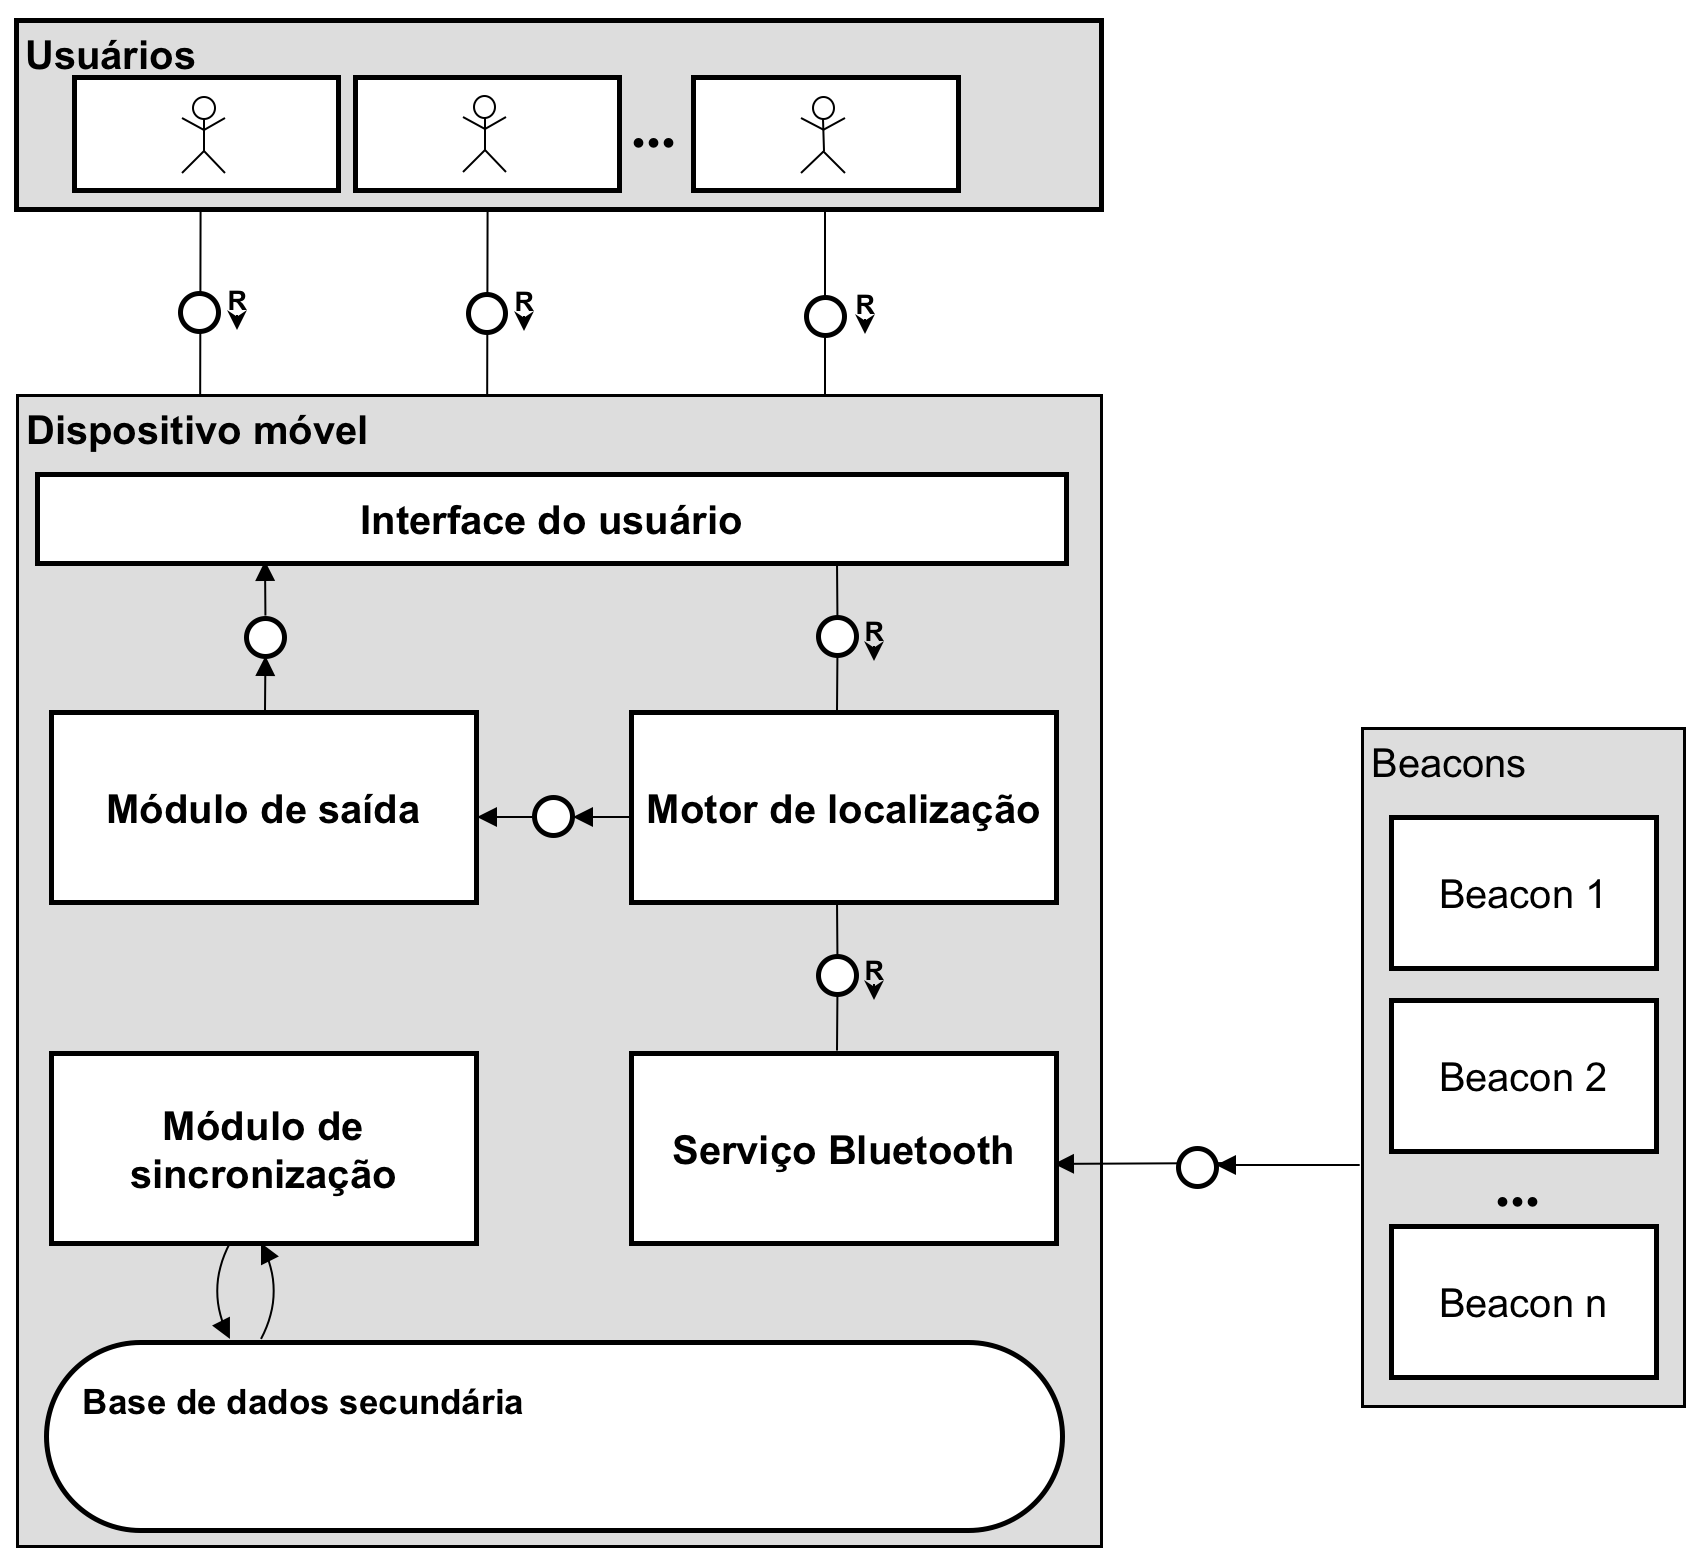
\includegraphics[width=\textwidth]{imgs/arquiteturaAplicativo.png}
		\fonte{Elaborado pelo autor.}
	\end{minipage}
\end{figure}

		\subsubsection{Módulo de sincronização}
Para que o aplicativo possa ser usado sem a exigência de conexão constante com a internet existe o módulo de sincronização. Ele é o responsável por manter a base de dados do aplicativo sempre atualizada em relação a base de dados principal do modelo, localizada no servidor, e tambem enviar as informações de monitoramento do aplicativo para o servidor.

O módulo se conecta com o servidor através do serviço web e verifica se existem modificações nos locais ou nos beacons desde a ultima sincronização e, em caso positivo, copia as novas informações até que as duas bases estejam equiparadas. Por padrão, a verificação em busca de modificações ocorre semanalmente, de forma a não consumir muito da bateria dos dispositivos. Todavia, esse valor pode ser ajustado para mais ou para menos afim de permitir que o modelo lide com mudanças dinâmicas no ambiente. A habilidade de suportar mudanças dinâmicas no ambiente é, segundo\citetexto{quinones2011supporting}, uma característica muito importante num sistema de localização acessível, visto que caminhos já conhecidos pelos usuários podem sofrer alterações, mesmo que levemente. Mudanças dinâmicas são alterações não previstas em rotas ou locais, como por exemplo um elevador não funcionando, uma sala fechada para limpeza, um caminho em manutenção, etc.

A execução da sincronização é independênte do usuário, sendo relizada de forma automatica e transparente, através de uma conexão com o servidor via internet, usando o padrão REST para troca das informações.

		\subsubsection{Base de dados secundária}
É função principal da base de dados secundária manter uma cópia das informações do servidor, bem como dados relativos as preferencias do usuário. Esses dados ficam armazenados locamente no dispositivo, numa base de dados SQLite. Exemplos de informações mantidas por esta base são as informações completas referentes aos becons e locais cadastrados no servidor e também os locais marcados pelo usuário como seus favoritos.

Além da função principal, a base secundária tambem guarda informações anonimas que visam permitir uma execução otimizada do aplicativo, tais como histórico completo de sincronizações realizadas, e dados de monitoramento do aplicativo, destinos selecionados pelo usuário, como rotas traçadas pelo sistema, instruções dadas ao usuário, informações de tempo e hora de uso, entre outras. Para garantir a privacidade do usuário, todas as informações analiticas do aplicativo são anonimizadas.

A base secundária é alimentada pelo módulo de sincronização, responsável por adicionar ou excluir os dados cadastrados. Seu objetivo é aumentar a usabilidade do aplicativo, não exigindo conexão com a internet para traçar as rotas, tornando mais rápida a resposta ao usuário.

		\subsubsection{Motor de localização}
O motor de localização é, juntamente com o serviço Bluetooth, o coração do modelo. Sua função receber os dados enviados pelo serviço Bluetooth juntamente com as requisições do usuário, e então calcular a rota desde a localização atual do usuário até o destino por ele escolhido.



A forma com que a rota é disponibilizada ao usuário ...
\citetexto{quinones2011supporting} busca entender, através de entrevistas, como PDV realizam seus deslocamentos diários, bem como elencar requisitos necessários para desenvolver sistemas que os auxiliam nesta tarefa. O trabalho afirma que PDV criam mapas mentais ricos em detalhes dos locais que mais frequentam, memorizando rotas e marcos específicos destes locais. 

Uma vez que o aplicativo é ativado, sua localização é obtida e informada a ele através do uso de voz




\citetexto{montague2010accessible}:

preparation, decision or confirmation. Preparation statements are instructions given as a lead up to an action the user would have to carry out. Decision statements are a call for action from the user following the instructions, occurring at decision points in the route. Confirmation statements are provided to reassure the user that they have carried out the previous step correctly.
Regardless of statement type there seemed to be a consistent structure: Action, Context and Reference (ACR) as shown in Figure 1.
The action gives meaning to the instruction the user is to carry out, such as “Look for...” and “Turn to the ...”. Context gives direction to the user -- Left, Forward, Up and so on. Finally, reference can be used to name objects or locations to assist the user such as Sofas, Fire exit, Stairwell etc. References are not always required.









	\subsubsection{Serviço Bluetooth}
O serviço Bluetooth é a perte do aplicativo onde está toda a programacão que o torna compativel com a tecnologia Bluetooth Low Energy. Através dele é feita a detecção dos beacons presentes no entorno do usuário, permitindo com que sua localização atual seja obtida.

Detecta quando usuário chega e manda um notificação

Beacons apenas em pontos chave. 

Bluetooth não precisa parear.

Beacons therefore add a layer of context. Previously, context was given by a user's details and history, combined with factors like time and possibly approximate location from GPS (think of Google maps and other local services). Now that can be enhanced by precise, immediate location and therefore movement, for example - entering the building, at a specific car in the showroom, at a particular gate in the airport, in a certain section of stadium seating, at some museum exhibit, walking towards a certain store and so on.
This creates opportunities for new types of app providing information, utility and convenience for users that wasn't previously possible. However it also generates significant quantities of data on movements and habits of consumers - this is a potential boon for companies, but is also likely to lead to privacy concerns, even though some companies already track location by GPS and wifi with consumer opt-in.
This means that the applications that emerge in the near future, and how they handle the balance of providing consumer utility with data collection, are going to be of crucial importance in promoting adoption of the technology. Supermarket (and other) loyalty cards show that it's possible to get this right - they are widely embraced, probably because the benefits to the consumer are clear and the proposition is simple.


	\subsubsection{Módulo de saída} % INDOOR HUMAN NAGIVATION SYSTEMS: visual, audio, haptic

\citetexto{ullman2009accommodating} 
 emphasized the importance of clear audible messages and spatial message elements 


A user study comparing a variety of interfaces (namely, spoken, tone outputs, compass or haptic inputs) [10] showed that the superiority of spoken directions (in combination with the compass) for a navigation task in an obstacle-free outdoor campus area.


Beep pra chamar atenção
Voz gerada por computador permite respnder mais rapidamente a mudanças no ambiente, não exigindo que falas passem por todo o processo de gravação.

Less is more. Simple and concise instructions were preferred over frequent and absolute ones, and using instructions only at significant waypoints was an effective strategy as the station’s unique sounds and a user’s instinct also helped navigation. It also proved that there was no need to communicate distance in metres or number of strides.

		\subsubsection{Pedido de ajuda}



\citetexto{dias2015navpal} If lost or disoriented, they typically ask for assistance from sighted people in the vicinity... In addition, if needed, the tools can assist the traveler in seeking assistance from others in the environment or guiding the traveler to safety....

Since we do not envision technology solutions completely eliminating the need for seeking human assistance in the future,



	\subsection{Componentes do servidor}
Nesta seção são apresentados cada um dos componentes, mostrados na figura \ref{fig:arquiteturaServidor}, que formam a arquitetura do servidor do modelo Insight.

\begin{figure}
	\caption{Diagrama de blocos da arquitetura do servidor}
	\label{fig:arquiteturaServidor}
	\centering%
	\begin{minipage}{.8\textwidth}
		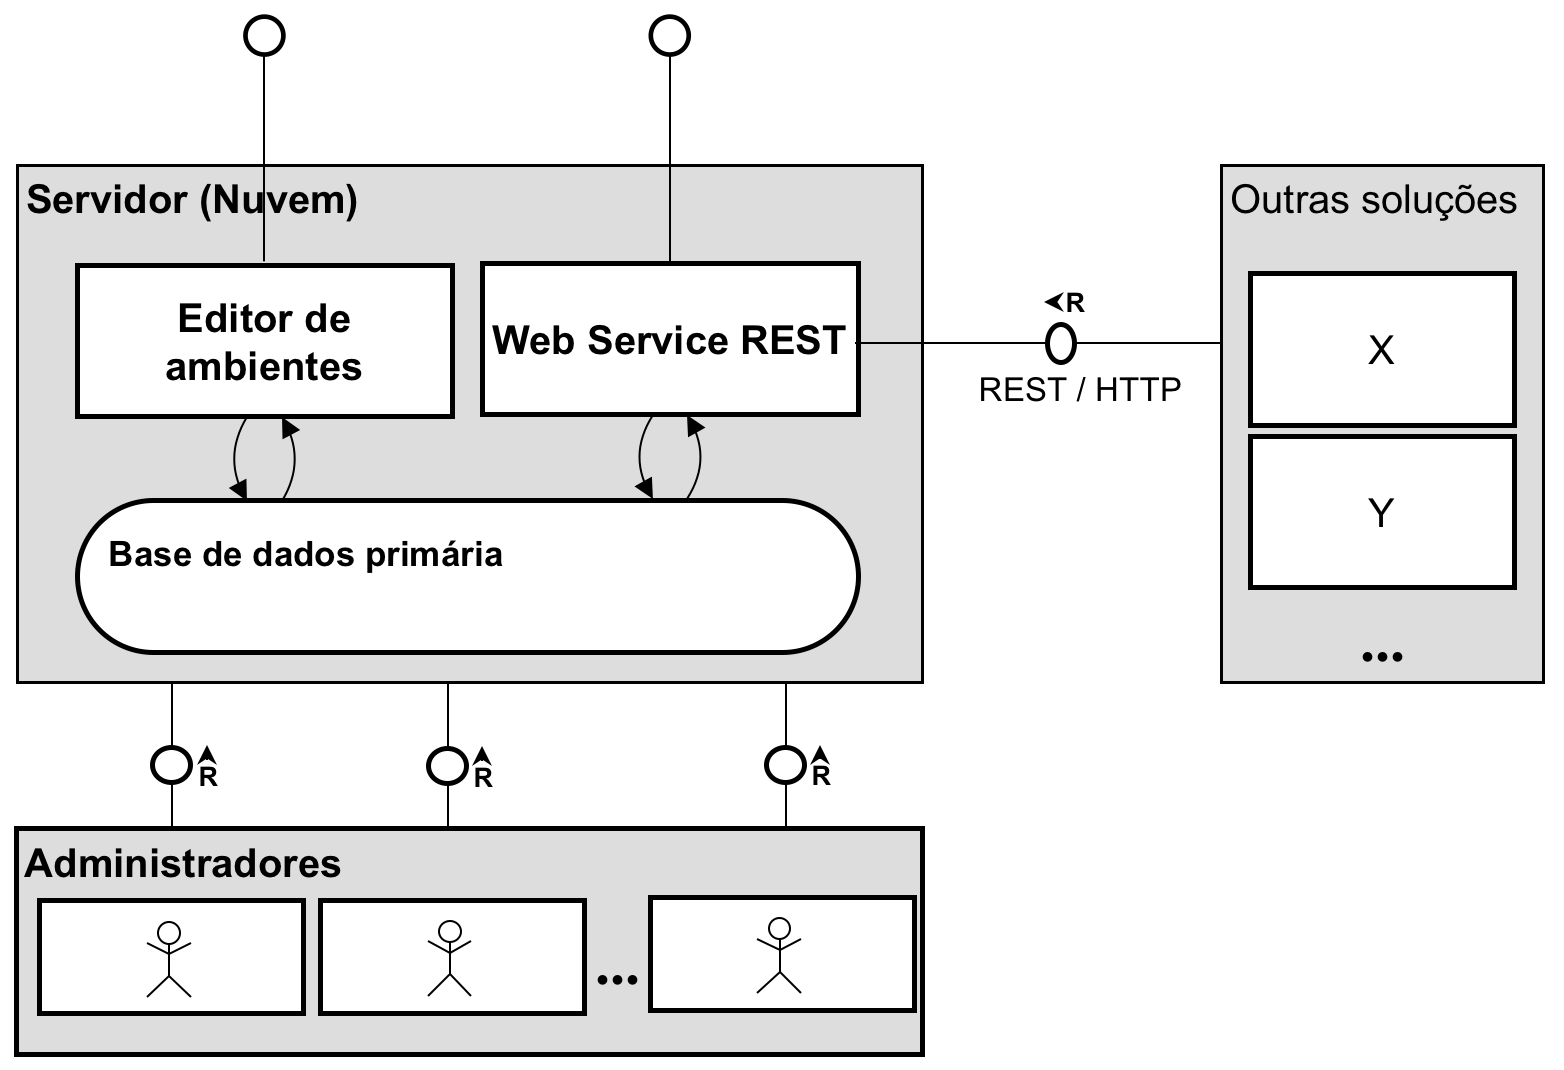
\includegraphics[width=\textwidth]{imgs/arquiteturaServidor.png}
		\fonte{Elaborado pelo autor.}
	\end{minipage}
\end{figure}

		\subsubsection{Serviço Web}

			Permite responder a ambientes dinâmicos


		\subsubsection{Base de dados principal}

%=======================================================================
% Metodologia
%=======================================================================
\chapter{Metodologia}
Enquadrando o presente trabalho na classificação apresentada em \citetexto{Gerhardt2009}, quanto à natureza da pesquisa, ele se caracteriza como uma pesquisa aplicada, pois objetiva gerar conhecimentos para aplicação prática dirigidos à solução de um problema específico que é a navegação e localização de deficientes visuais. A abordagem do trabalho é qualitativa e, do ponto de vista dos objetivos, é uma pesquisa exploratória e descritiva, buscando resultar em um modelo acessível de localização e navegação em ambientes internos. O procedimento técnico utilizado para a construção da pesquisa é a pesquisa bibliográfica.

	\section{Desenvolvimento}
O trabalho de modelagem e desenvolvimento do Insight foi divido em 9 passos metodológicos apresentados na figura \ref{fig:passosMetodologicos}. Os passos 1 a 6 foram realizados no presente trabalho. Os demais passos serão realizados na disciplina Trabalho de Conclusão II, que também compreende os requisitos para a colação de grau da Universidade do Vale do Rio dos Sinos (UNISINOS).

\begin{figure}[!ht]
	\caption{Passos metodológicos}
	\label{fig:passosMetodologicos}
	\centering%
	\begin{minipage}{.7\textwidth}
		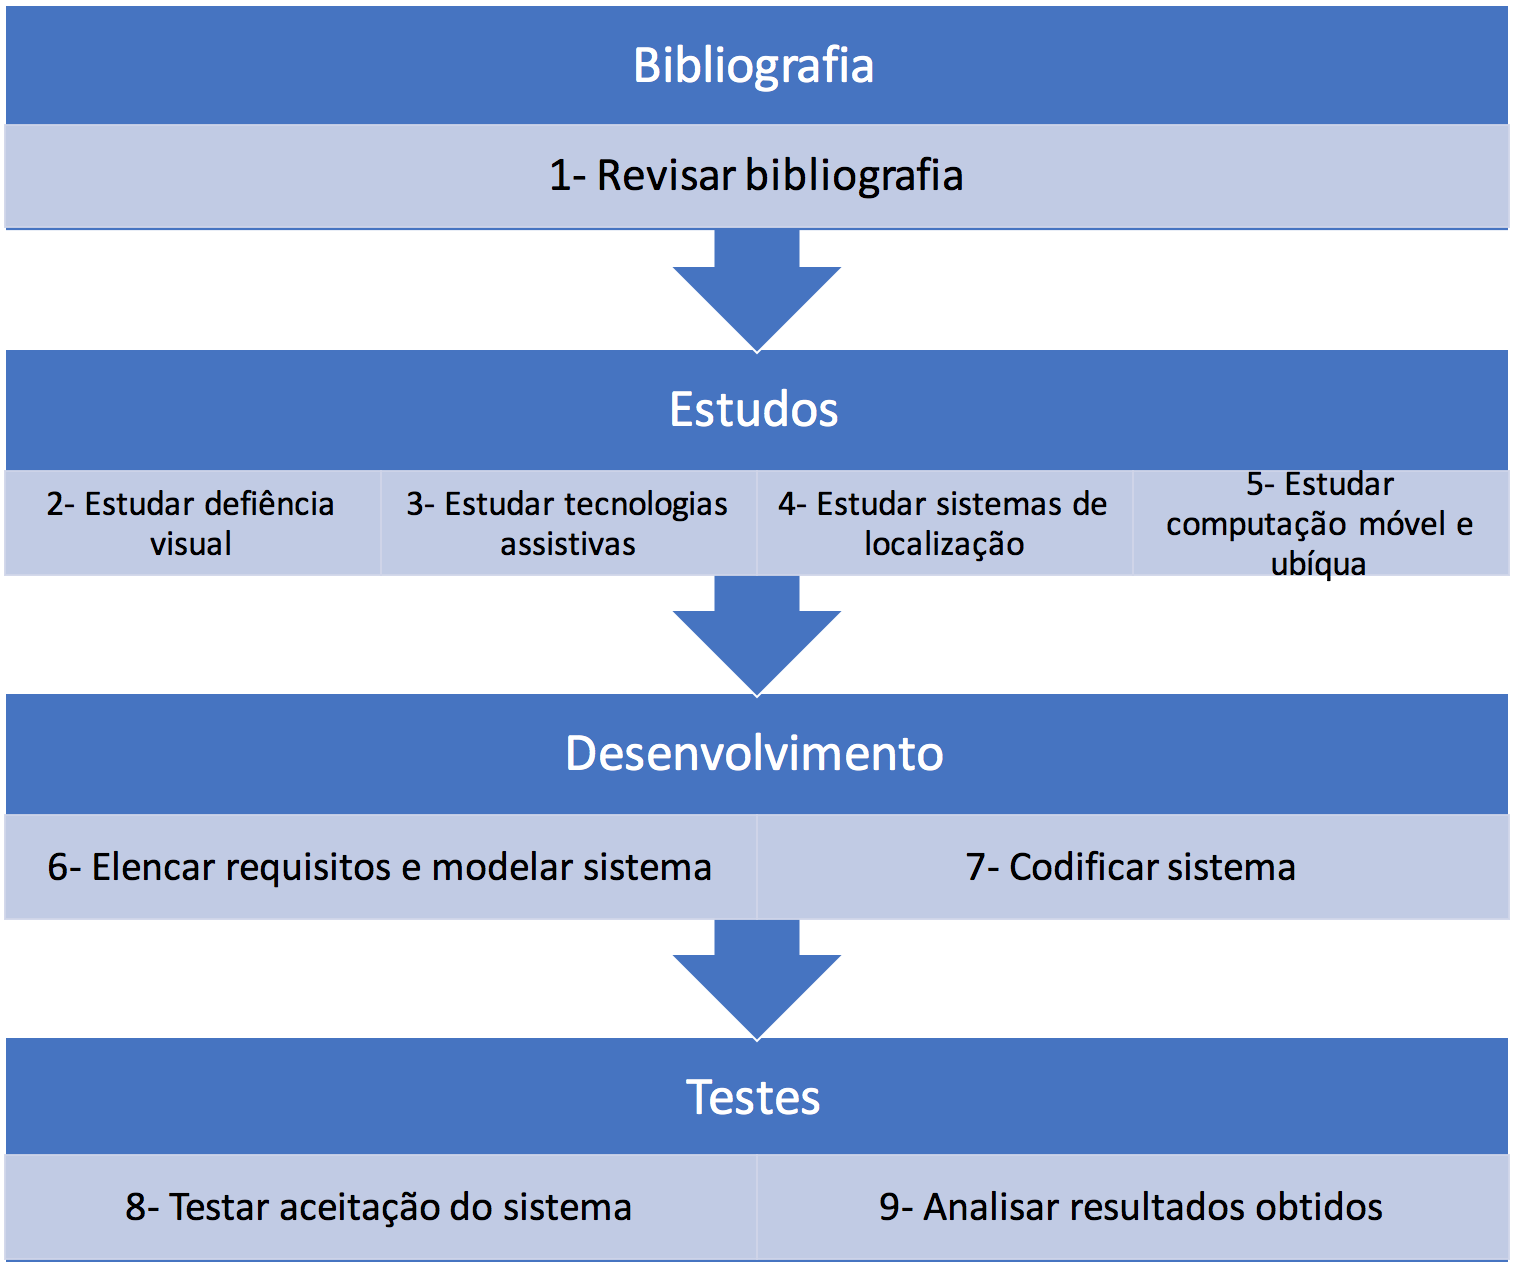
\includegraphics[width=\textwidth]{imgs/passosMetodologicos}
		\fonte{Elaborado pelo autor.}
	\end{minipage}
\end{figure}

A seguir são apresentados brevemente cada um dos passos concebidos:

% passos
\begin{enumerate}
	%	1
	\item \textbf{Revisar bibliografia:} Pesquisa bibliográfica objetivando descobrir trabalhos envolvendo o tema em questão. Realizar leitura e resumo dos trabalhos relevantes encontrados, e, com isso, criar uma fundamentação teórica adequada para o desenvolvimento desta pesquisa.
	%	2
    \item \textbf{Realizar estudo sobre deficiência visual:} Estudar essa deficiência em busca de compreender a maneira com que ela afeta seus portadores, e também o processo mental realizado por eles durante seu deslocamento, tanto em ambientes familiares como desconhecidos, afim de criar uma abstração desse processo aplicando-a ao modelo.
	%	3
    \item \textbf{Realizar estudo sobre tecnologias assistivas:} Estudar e verificar quais tecnologias já foram aplicadas na acessibilidade, avaliando quais podem ser utilizadas no desenvolvimento do modelo para melhor atender às necessidades dos PDV.
	%	4
    \item \textbf{Realizar estudo sobre sistemas de localização:} Estudo buscando compreender o estado da arte dos sistemas de localização, identificando características que devem ser aplicadas em um sistema acessível destinado a PDV.
	%	5
    \item \textbf{Realizar estudo sobre computação móvel e ubíqua:} Estudar o conceito de computação ubíqua, bem como conceitos relacionados, em busca de ideias que podem ser aplicadas no desenvolvimento e no uso do presente modelo, tornando-o mais natural e transparente possível aos usuários.
    %	6
    \item \textbf{Elencar requisitos e modelar o sistema:} Elaborar os modelos necessários para o posterior desenvolvimento do sistema, utilizando a linguagem UML.
    %	7
    \item \textbf{Codificar sistema:} Codificar o sistema de acordo com a modelagem realizada.
	%	8
	\item \textbf{Testar aceitação do sistema:} Codificar uma prévia do modelo desenvolvido de modo que ela possa ser avaliada em campo.
	%	9
	\item \textbf{Analisar resultados dos testes:} Realizar análise dos resultados obtidos através dos questionários, traçando uma conclusão do trabalho desenvolvido. Posteriormente, verificando os benefícios e dificuldades apresentados pelo sistema aos participantes, afim de estabelecer ajustes e correções, bem como trabalhos futuros.
\end{enumerate}

	\section{Avaliação}
A avaliação do modelo proposto se dará após a implementação e implantação do sistema. Para a implantação dele serão convocados usuários PDV com interesse em colaborar com a pesquisa. Os usuários utilizarão o sistema e posteriormente o avaliarão usando duas técnicas distintas: a primeira será através de questionários anônimos durante o período de testes, afim de detectar problemas pontuais e verificar a adaptação do usuário ao sistema durante o período de uso; a segunda será a técnica da entrevista estruturada. 

A entrevista ocorrerá em dois momentos. Antes de iniciar o período de testes, para obter informações sobre a forma como os usuários se guiam quando necessitam deslocar-se em um ambiente desconhecido. Após o término dos testes, para obter informações relativas à qualidade da localização e da navegação oferecidas pelo protótipo. O resultado da análise permitirá identificar a eficácia do sistema e possibilitará elencar melhorias e/ou trabalhos relacionados ao tema.

(TODO: avaliação por cenários ou usuários)

\chapter{Conclusão}

\section{Comparação entre os trabalhos estudados e o modelo proposto}

\FloatBarrier
\begin{table}
	\caption{Tabela comparativa entre os trabalhos relacionados e o Insight}
	\label{tab:trabalalhosRelacionadosEInsight}
	\centering%
	\begin{minipage}{1\textwidth}
		\begin{tabular}{ | p{3cm} | p{3cm} | p{3cm} | p{3cm} | p{3cm} | }
			\hline
										& Percept 									& UCAT 								& Navigation System for Work Zones		& Tirésias   \\ \hline
				Método de localização 	& RFID 										& Bluetooth 2.1 					& Bluetooth 4.0 						& GPS 						 \\ \hline
				Abrangência 			& Indoor 									& Indoor e outdoor 					& Zonas em obras 						& Indoor 					 \\ \hline
				Ambientes dinâmicos		& Não especificado							& Não especificado					& Não especificado						& Não especificado			 \\ \hline
				Hardware específico 	& Sim 										& Não 								& Não 									& Não 						 \\ \hline
				Comunicação 			& Internet ou intranet 						& Internet 							& Internet 								& Internet ou intranet 		 \\ \hline
				Interoperabilidade 		& Não 										& Não 								& Não 									& Sim 						 \\ \hline
				Banco de dados 			& Postgres 									& SQLite 							& MySQL 								& Não especificado 			 \\ \hline
				Linguagem 				& Java 										& Java 								& Java 									& Objective-C 				 \\ \hline
				Sistema operacional 	& Android 									& Android 							& Android 								& iOS 						 \\ \hline
				Hardware 				& Luva equipada c/ leitor RFID e smartphone & Dispositivos móveis c/ Bluetooth 	& Dispositivos móveis c/ Bluetooth 		& Dispositivos Móveis c/ GPS \\ \hline
				Arquitetura 			& Cliente-servidor 							& Cliente-servidor 					& Cliente-servidor 						& Cliente-servidor 			 \\ \hline
		\end{tabular}
		\fonte{Elaborado pelo autor.}
	\end{minipage}
\end{table}
\FloatBarrier
	
	\section{Trabalhos futuros}
- Considerar dificuldade do percurso
- Wearables pra não ser necessário usar as mãos \\
- Salas de aula, integração 

%=======================================================================
% Referências
%=======================================================================
\bibliography{bibliografia}

\end{document}